% simple.tex - simple Master's thesis sample
% $Id: simple.tex 309 2011-01-28 14:46:48Z vlado $
%\documentclass[12pt]{dalcsthesis}
% to prepare draft version use option draft:


\documentclass[12pt]{dalcsthesis}

\usepackage[pdftex]{graphicx}

\usepackage{epstopdf}
\usepackage{epsfig}
\usepackage{verbatim}
\usepackage{amsmath}
\usepackage{amssymb}
\usepackage{adjustbox}
\usepackage{tabularx}
\usepackage{subfigure}
\usepackage{algorithm2e}

\usepackage{url}
%\usepackage{caption}
%\captionsetup[table]{skip=10pt}

\begin{document}

\mcs  % options are \mcs, \macs, \mec, \mhi, \phd, and \bcshon
\title{Feature Based adaptive motion model}
\author{Rohan Bhargava}
\defenceday{1}
\defencemonth{October}
\defenceyear{2013}
\convocation{January}{2014}

% Use multiple \supervisor commands for co-supervisors.
% Use one \reader command for each reader.

\supervisor{Dr. Thomas Trappenberg}
\supervisor{Dr. Mae Sato}
\reader{D. Odaprof}
\reader{A. External}
\providecommand{\tabularnewline}{\\}
\newcommand{\lyxdot}{.}
%\nolistoftables
%\nolistoffigures

\frontmatter


\begin{abstract}
\begin{comment}
We present a method to learn and adapt the motion model. The motion model can be influenced by environmental properties and is a crucial part of the navigation system.Examples are the drift that is accounted in the motion model can be different for carpets and tiles. The AUV can have a change in their motion model when they are moving from fresh water to sea water. Our algorithm is based on the Expectation Maximization Framework which help us to learn the right parameters for the model.
The Expectation Step is completed by particle filtering and smoothing. The Maximization step involves finding the parameters for the model.We use side sonar images to extract landmarks which can gives us position estimates to help us evolve our motion model.This leads to a better position estimate of the robot. 
We found that the our learning motion model adapted well to the change in parameters and had low localization error compared to static motion model. 
This algorithm eliminates the need for laborious and hand-tuning calibration process. The main significance of learning the motion model is to have better navigation algorithms and also its a step towards robots being able to adapt to environment without human intervention.
We validate our approach by recovering a good motion model when the density,temperature of the water is changed in our simulations.
\end{comment} 
\end{abstract}

\begin{acknowledgements}
Thanks to all the little people who make me look tall.
\end{acknowledgements}

\mainmatter

\chapter{Introduction}
 





\section{Motivation}
The core of human environment interaction is the ability of a person to know its position in surrounding environment. The process of estimating the robot's position and orientation in the world is termed as Localization \cite{thrun2005probabilistic}.  A common approach to determine the location of a robot is through the use of Global Positioning System (GPS), a series of satellites in low earth orbit that use differential positioning to determine a location for a receiver.  Another approach is to provide a prior map of the environment and with help of sensors a robot perceives the world and localizes itself in it. An additional challenge to localization is when sensing external environment is impossible or incomplete due to unreliability and inaccessibility of the sensors. In this case the localization estimate can be updated using self-generated cues such as acceleration and velocity.  

An example for such a scenario from underwater robotics is maintaining a pose estimate of an Autonomous Underwater Vehicle(AUV), such as Hugin 4500 (Figure ~\ref{fig-Hugin 4500}). In AUV the pose estimation relies on Inertial Navigation Systems (INS) which gives an estimate of the velocity, position and orientation.  All INS systems suffer from drift i.e. small errors in measurement of acceleration and angular velocity are integrated into progressively larger error.  To compensate for drift systems such as Doppler Velocity Log (DVL), surface GPS etc. are used \cite{Lammas2004} \cite{leonard1998autonomous}. Hegrenaes et al \cite{Hegrenæs2008} pointed out that there are situations where these systems fail or readings from these sensors need to be discarded due to poor quality.  An example of such a situation is the non-feasibility of the vehicle to surface.  In such situations they proposed to use the self-generated velocity estimates to aid INS systems. 
\begin{figure}
  \centering
     {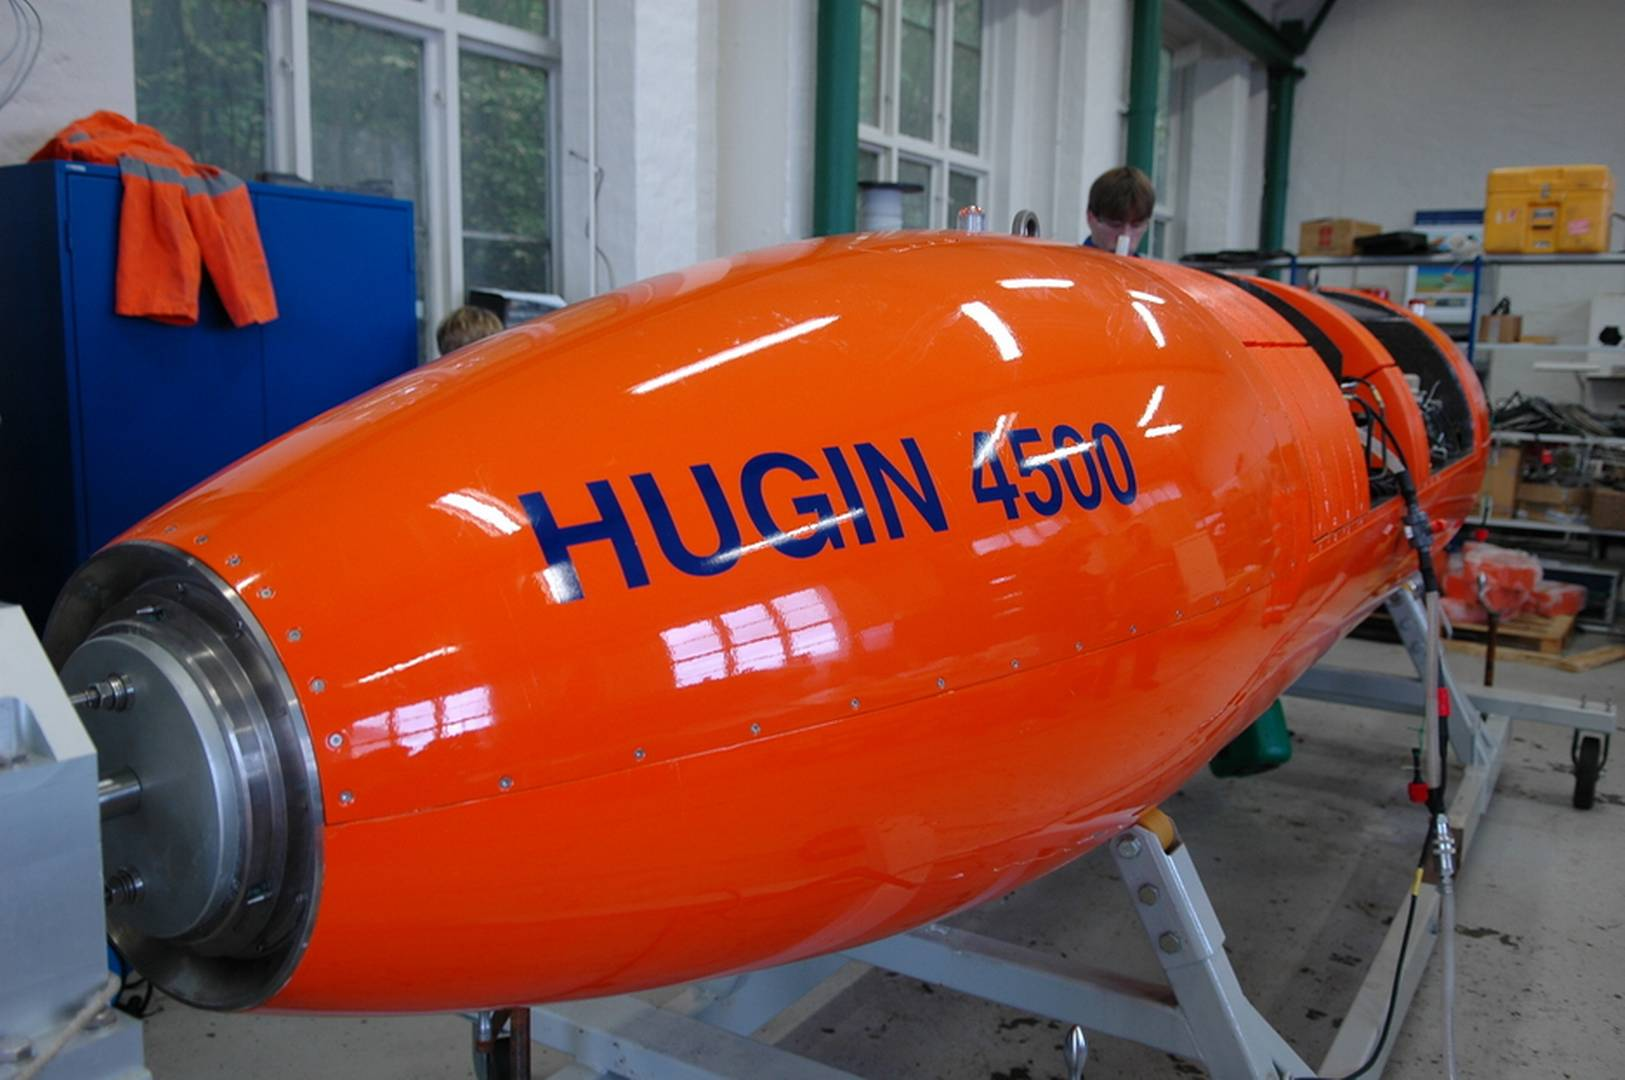
\includegraphics[height = 3.0 in]{../hugin_4500.png}}
  \caption{\label{fig-Hugin 4500} Hugin 4500 autonomous underwater vehicles. When submerged, the vehicle uses dead reckoning, incorporating DVL and compass input to maintain an estimate on current positioning.
}
\end{figure}


The estimates can be difficult to acquire and maintain due to uncertainties in way a robot interacts and senses its environment. These uncertainties can arise due to noisy and incomplete sensing of the environment, uncertain movements of a robot in the environment and changes in the environment itself.  To address these issues Sebastian Thrun \cite{thrun2005probabilistic} represented the motion and sensor models probabilistically. He defines it as, instead of relying on single ''best guess" as to what might be the case, probabilistic algorithms represent the information by probability distributions over a whole space of guesses.  To update the state of a robot probabilistically there are algorithms such as Kalman Filter \cite{kalman1960new}, Particle Filter \cite{gordon1993novel} etc. which are based on Bayes filter. 

In probabilistic robotics the motion and sensors models are represented by a distribution which is defined by its parameters.  The process of determining parameters to kinematic model is termed as calibration \cite{cox1990autonomous} \cite{vukobratovic1989introduction}. Generally the parameters to the models are hand tuned and are derived by conducting calibration experiments. Such calibration methods are impractical for two reasons. Firstly these processes are labour intensive and require prior information about the environment and robot. Secondly, changes in robot (e.g.-:  general wear and tear) and environment (e.g.-: moving from fresh water to sea water) leads to changes in the parameters. The changes in underwater environments can be due to change in density, temperature etc. of water. These changes require recalibration of a robot while it is in operation which in most cases is not possible to do. The inaccuracies in the models will effect results for higher level tasks such as path planning \cite{Lav06}, Simultaneous Localization and 
Mapping (SLAM) \cite{thrun2005probabilistic} \cite{grisettiyz2005improving} etc.

Roy and Thrun \cite{Roy} proposed an online calibration method for land robots which can be performed without human intervention.  They approached the calibration process as maximum likelihood estimation problem which gives an estimate of parameters for the given data. The calibration parameters are iteratively estimated by comparing pair of subsequent sensor readings. The algorithm proposed worked well for systematic drifts and the results showed the position error reduced by approximately by 83 "\%".

Alizar and Parr \cite{Eliazar2004} continued the work further by estimating non-systematic drifts.  They proposed an algorithm to learn the right parameters of a motion model for a land robot using Expectation Maximization Framework \cite{dempster1977maximum}. It is an unsupervised machine learning technique that alternates between the expectation and maximization step. In the Expectation Step it creates an expectation of the log-likelihood using the current estimate of the parameters and the Maximization step which computes parameters maximizing the expected log-likelihood found in the Expectation Step. They were able to learn accurate motion models with very little user input.

Yapp \cite{Yap2008} took Alizar and Parr's \cite{Eliazar2004} work further and proposed an algorithm to learn the motion and sensor models for land robots. They used the same Expectation Maximization framework to learn the right parameters for the models. To calculate the likely trajectory of a robot both the algorithms implemented particle filtering \cite{ristic2004beyond} \cite{chen2003bayesian} and smoothing \cite{doucet2000monte}.  The algorithm started with an estimate of initial parameters and iteratively optimized the parameters based on the data collected during robot's operation. The algorithm assumed that a prior map of the environment is provided. 

In my thesis I specifically deal with water environments such as oceans, rivers etc. which are highly dynamic.  The algorithm proposed here is different from the work done before in two ways. Firstly the algorithm is meant to learn the right parameters for an AUV's motion model. Secondly, the algorithm can learn motion model for unknown environments by generating landmarks using side sonar images and therefore doesn't have to rely on static maps. Sound Navigation and Ranging (SONAR) is a technique based on sound propagation used for detecting objects underwater. Side scan sonar is a specific type of sonar used to image the topography of a sea floor.  The SONAR sensor is the only imaging tool that can work at high depth. 

My algorithm uses EM algorithm to calculate the most likely parameters for a data set.  The trajectories are calculated by implementing particle filtering and smoothing.  Particle Filters are chosen because they can mode non-linear transformations as well as have no restrictions in model. Particle smoothing was performed because Russel and Norving ~\cite{russell2003artificial} pointed out that the state of the system is better estimated by smoothing as it incorporates more information that just filtering. 

The remainder of the thesis is structured as follows. Chapter 2 will explain the motion model for AUV as well as give an insight on particle filtering and smoothing. Chapter 3 will give an overview of Expectation Maximization and show how this framework is used to adapt parameters for a motion model. Chapter 4 will give explain how landmarks are extracted from side sonar images. The reliability of the landmarks are shown by extracting motion information and the algorithm to do that is described in Chapter 4. Chapter 5 consist results of a simulated experiment to show the effectiveness of the algorithm. This chapter also includes the comparison of motion estimation using side sonar images to DVL.
 
\begin{comment}
 The core of human environment interaction is the ability of a person to know its position in surrounding environment. The process of estimating robot's position and orientation in the world is termed as Localization \cite{thrun2005probabilistic}. It is the answer to the question ''Where am I?”. The current location of a robot can be determined by Global Positioning Systems, landmarks, maps etc. A common approach is to provide a prior map of the environment and a robot with help of sensors perceives the world and localizes itself in it. Another way to estimate the position of a robot is by knowing how a robot moves in the world . For example by knowing at what velocity a robot is moving we can predict its future location. There are various algorithms such as Particle Filter \cite{gordon1993novel},Kalman Fitler \cite{kalman1960new} etc. to estimate the state of a robot. The way the robot moves and senses the world are captured in motion and sensor models. These models are basic building blocks to various 
algorithms such as path planning \cite{Lav06}, Simultaneous Localization and Mapping (SLAM) \cite{thrun2005probabilistic} \cite{grisettiyz2005improving}  etc. which require an accurate estimate of robot's position. 

In order to account for the uncertainty in motion Sebastian Thrun \cite{thrun2005probabilistic} represented the models probabilistically. Eliazar and Parr \cite{Eliazar2004} pointed out that the essential input are the parameters to these models. The process of determining the parameters to a kinematic model is termed as calibration. Generally the robot is calibrated at the start of the experiment and the parameter values are not changed throughout the experiment. In practice wherever there is a significant change in the environment, robots are manually re calibrated during the experiment. In most of the cases it is not possible to recalibrate while the robot is in operation. As our environments are dynamic our models need to adapt to them. Eliazar and Parr \cite{Eliazar2004} proposed an algorithm to learn parameters of a motion model for land robots. Teddy Yapp \cite{Yap2008} took the work further and learned parameters for motion and sensor models for land robots. Both of their algorithms used 
Expectation Maximization framework to learn right parameters for models.

For my thesis I specifically deal with water environments such as oceans, rivers etc. which are highly dynamic and will lead to changes in motion model for Autonomous Underwater Vehicle. A specific application to demonstrate the importance of accurate motion model is Navigation. In AUV navigation relies on Inertial Navigation System(INS) which gives an estimate of velocity, position and orientation. All INS systems suffer from drift i.e. small errors in measurement of acceleration and angular velocity are integrated into progressively into larger error. Hegrenaes et al \cite{Hegrenes2008} pointed out that systems such as Doppler Velocity Log(DVL), surface GPS etc are used to compensate for the drift but they are situations where these systems fail or readings are discarded due to poor quality. To solve this particular problem they used velocity estimate from a static motion model to aid INS systems. In my thesis I propose an online system for an AUV to adapt its motion model to the dynamic environment which 
can be used for applications such as navigation as well as automate the calibration process. 

In Chapter~\ref{learning the motion model} I demonstrate how the parameters of a motion model can be estimated during its normal operation. The algorithm uses machine learning methods to learn the parameters as well as eliminate the necessity of identifying the parameters through a manual laborious calibration process. Yapp \cite{Yap2008} in his algorithm used Expectation Maximization \cite{dempster1977maximum} framework to estimate the right parameters for the model and I use the same framework for my algorithm. It is an unsupervised machine learning technique primarily used to estimate parameters. It alternates between the Expectation Step which creates an expectation of the log-likelihood using the current estimate of the parameters and the Maximization Step which computes parameters maximizing the expected log-likelihood found in the E step. 

In the algorithm proposed by Yapp \cite{Yap2008} to calculate the likely trajectory of a robot particle filtering \cite{ristic2004beyond} \cite{chen2003bayesian} and smoothing \cite{doucet2000monte} \cite{doucet2009tutorial} were performed using the sensor data collected during robot's normal operation. The particle filters were chosen because they can model non-linear transformations as well as they have no restrictions in model. Particle smoothing was performed because Russel and Norving \cite{russell2003artificial} pointed out the state of the system is better estimated by smoothing as it incorporates more information than just filtering. The maximum likelihood estimate of the parameters given the robot's trajectory and the motion data is calculated. The algorithm by Yapp \cite{Yap2008} was for land robots as well as assumed a prior map of the environment.  

The algorithm proposed in this thesis is for an AUV and can learn the motion model in unknown environments. In the algorithm instead of using a static map we used landmarks. In AUV the landmarks are extracted from side sonar images and are collected as sensor data. The algorithm assumes that the robot is equipped with a side sonar sensor and has access to its noisy motion data. Sound Navigation and Ranging (SONAR) is a technique based on sound propagation used for detecting objects underwater. The SONAR sensor is the only imaging tool which can work at high depth. Side scan sonar is a specific type of sonar used to image the topography of the sea floor.

To summarize I am proposing an algorithm to learn the right parameters of a motion model for an AUV. The parameters are learned on the fly without having a prior map or revisiting places. Results of the simulated experiment are presented in chapter ~\ref{results} to show the effectiveness of the algorithm. 
\end{comment}


 

\section{Contributions}
The main contribution of the work presented here is to provide an algorithm to adapt the motion model for AUV. The automated process of calibration of the robots gets rid of hand tuning of the models and gives us an online process which can be performed during the robot's mission. 
  
\begin{comment}
The main contributions of the algorithm are-:

1) \textbf{Adaptive Motion Model}-: The motion model for AUVs adapt to changing environment. This automated process of calibration of the robots lead to no hand tuning of the models and gives us an online process which can be preformed during the robot's mission.  

2) \textbf{Motion Estimation from Side Sonar Images}-: We present an approach to estimate the movement from side sonar images which can be coupled with existing motion model and can improve localization. It can be easily be performed on-board as limited amount of interest points are used which lead to lesser computation and memory usage. 
\end{comment}
\chapter{Background}
In the chapter we start by discussing how motion models are probabilistically represented as well as give an insight about motion models for AUV. This helps us in understanding of how motion model captures the probabilistic movements of robots. We then discuss a probabilistic state estimation algorithm such as particle filter \cite{ristic2004beyond} \cite{chen2003bayesian} which is at the heart of my algorithm as well as many other robotics systems. Lastly we discuss about particle smoothing \cite{doucet2000monte} \cite{doucet2009tutorial} which gives an estimate of ground truth by calculating the distribution of past states with taking into account all the evidence up to present. 

\section{Motion Model}
\label{chap-:Motion Model}
A motion model is responsible for capturing the relationship between the control input and the change in robot's configuration. Thrun \cite{thrun2005probabilistic} models the motion of a robot probabilistically because the same
control inputs will never reproduce the same motion. A good motion model will capture the errors such as drift that are encountered during the motion of a robot. The motion model is a necessary ingredient of many algorithms such as localization,mapping etc. 

Let $X=(x,y,\theta)$ be the initial pose of the robot in x-y space. Mathematically the motion model can be described as $P(X^{'}|X,u)$, where $X^{'}$ is the pose after executing the motion command $u$. Based on the control input Thrun \cite{thrun2005probabilistic} divided the motion model in two classes 1) Odometry based motion model 2) Velocity based motion model.

The first class of motion models are used for robots equipped with wheel encoders. Odometry is generally obtained by integrating wheel encoders information and is more accurate than velocity.  
Velocity based models calculate the new position based on velocities and time elapsed. These models are implemented for Autonomous Underwater Vehicle(AUV) and Unmanned Aerial Vehicles(UAV). Both odometry as well as velocity suffer from drift and slippage therefore the same control commands will not generally reproduce the same motion.

The velocity motion model proposed by Thrun \cite{thrun2005probabilistic} assumes that robot can be controlled through two velocities a rotational and translational velocity. The translational velocity at time $t$ is denoted by $v_{t}$ and rotational velocity by $w_{t}$. Hence the control input $u_{t}$ can be represented by  
\begin{center}
$u_{t}=\bigl(\begin{array}{c}
                v_{t} \\
                w_{t}
               \end{array}\bigr)$
  
\end{center}

The assumption is that positive rotational velocities $w_{t}$ induce a counterclockwise rotation whereas positive translational velocities $v_{t}$ correspond to forward motion. The set of equations to compute the next state of a robot for a velocity motion model are 

\begin{equation}
x_{t}=x_{t-1}+V_{t-1}/W_{t-1} \sin(\theta_{t-1})+ V_{t-1}/W_{t-1} \cos(\theta_{t-1} + W_{t-1} \delta t)
\end{equation}

\begin{equation}
y_{t}=y_{t-1}+V_{t-1}/W_{t-1} \cos(\theta_{t-1})- V_{t-1}/W_{t-1} \sin(\theta_{t-1} + W_{t-1} \delta t)
\end{equation}

\begin{equation}
\theta_{t}=\theta_{t-1}+ W_{t-1} \delta t
\end{equation}
 

%Read about the mathematical derivation for the equation

In an AUV a velocity motion model is implemented and to represent AUV's motion, 6 independent coordinates are necessary to determine the position and orientation of the rigid body. The notations used for marine vehicles are described in Table \ref{marine notation}. 
%\begin{center}

\begin{table}[tbh]
\centering
\label{marine notation}
\begin{tabular}{|c|>{\centering}p{3cm}|>{\centering}p{3cm}|>{\centering}p{3cm}|>{\centering}p{3cm}|}
\hline 
DOF &  & forces and moments & linear and angular vel. & positions and Euler angles\tabularnewline
\hline 
\hline 
1 & motions in the x-direction (surge) & X & u & x\tabularnewline
\hline 
2 & motions in the y-direction (sway) & Y & v & y\tabularnewline
\hline 
3 & motions in the z-direction (heave) & Z & w & z\tabularnewline
\hline 
4 & rotation about the x-axis (roll) & K & p & $\phi$\tabularnewline
\hline 
5 & rotation about the y-axis (pitch) & M & q & $\theta$\tabularnewline
\hline 
6 & rotation about the z-axis (heave) & N & r & $\psi$\tabularnewline
\hline 
\end{tabular}
\caption{Notation used for marine vehicles. Table from \cite{Thor}}
\end{table}

%\end{center}



The pose of AUV can be represented as $s=(x,y,z,\theta,\phi,\psi)$. The first three coordinates correspond to the position along the x,y,z axes while the last three coordinates describe the orientation. Fossen \cite{Thor} in his book describes the motion of a marine vehicle in 6 DOF using two coordinate systems as shown in Figure ~\ref{fig-Coordinate System}. $X_0$, $Y_0$, $Z_0$ represent the moving coordinate frame and is called as body-fixed reference frame. The earth-fixed reference frame is denoted by $X$, $Y$, $Z$. The origin of the body-reference frame is denoted by $O$ and is chosen to coincide with the center of gravity denoted by $CG$.  

To estimate the position of an AUV we need to calculate the velocity at which the AUV is currently moving. The velocity can be computed in two ways-: 1) Static Motion model 2) Dynamic Motion model

Hegrenaes \cite{Hallingstad2007} points that a way to implement a simple static motion model as table look-up based on experimental data. 
\begin{equation}
\label{eq:static AUV model}
u_{r}=f(n_{s})
\end{equation}


$u_{r}$, $n_{s}$ are the water relative linear velocity in x direction and control system set point respectively. In a similar manner an expression can be established for $v_{r}$.

Another way to implement the motion model is through dynamics. The 6 Degrees of Freedom (DOF) rigid body equations of motion described by Fossen \cite{Thor} are \\
\begin{equation}
X=m[u^{.}-vr+wq-x_{G}(q^{2}+r^{2})+y_{G}(pq-r^{.})+z_{G}(pr+q^{.})]
\end{equation}

\begin{equation}
Y=m[v^{.}-wp+ur-y_{G}(r^{2}+p^{2})+z_{G}(qr-p^{.})+x_{G}(qp+r^{.})]
\end{equation}

\begin{equation}
Z=m[w^{.}-uq+vp-z_{G}(p^{2}+q^{2})+x_{G}(rp-q^{.})+y_{G}(rq+p^{.})]
\end{equation}

\begin{equation}
K=I_{x}p^{.}+(I_{z}-I_{y})qr-(r^{.}+pq)I_{xz}+(r^{2}-q^{2})I_{yz}+(pr-q^{.})I_{xy}+m[y_{G}(w^{.}-uq+vp)-Z_{g}(v^{.}-wp+ur)]
\end{equation}

\begin{equation}
M=I_{y}q^{.}+(I_{x}-I_{z})rp-(p^{.}+qr)I_{xy}+(p^{2}-r^{2})I_{zx}+(qp-r^{.})I_{yz}+m[y_{G}(u^{.}-vr+wq)-z_{g}(w^{.}-uq+vp)]
\end{equation}

\begin{equation}
 N=I_{z}r^{.}+(I_{y}-I_{x})pq-(q^{.}+rp)I_{yz}+(q^{2}-p^{2})I_{xy}+(rq-p^{.})I_{zx}+m[x_{G}(v^{.}-wp+ur)-y_{g}(u^{.}-vr+wq)]
\end{equation}


% need to find the best way to write these equations
\begin{figure}
  \centering
     {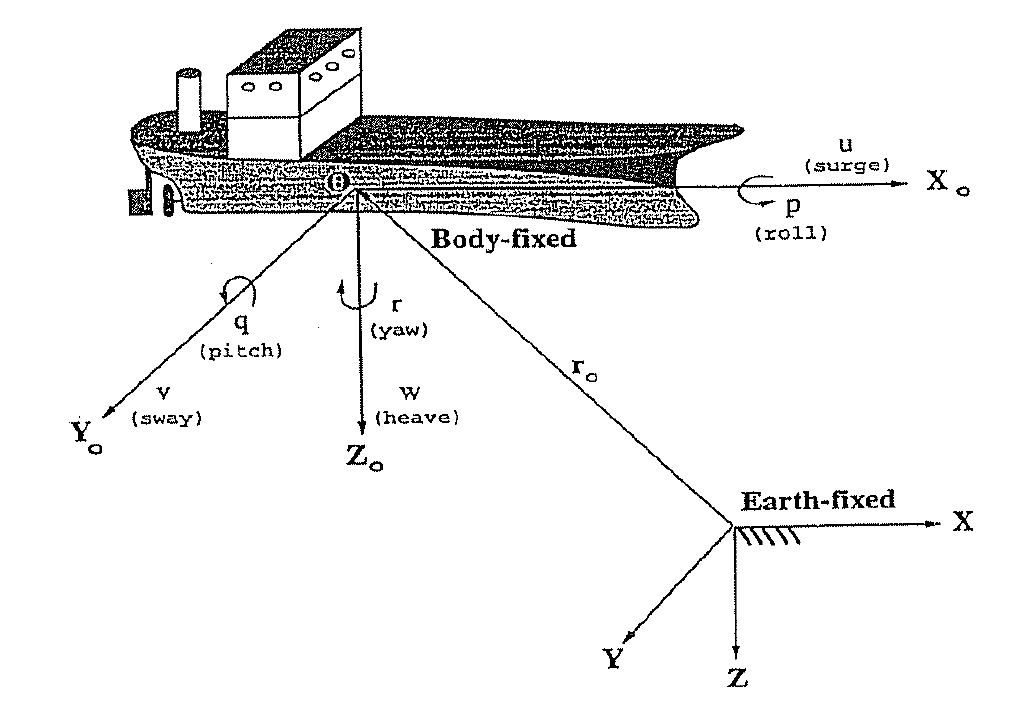
\includegraphics[height = 3.0 in]{/home/rohan/Documents/thesis/coordinate_system.png}}
  \caption{\label{fig-Coordinate System} Body-fixed and earth-fixed reference frames to describe the coordinate system of an AUV. Figure from \cite{Thor}
}
\end{figure}


The equations described above can be expressed in a more compact form: 
% what is RB
\begin{equation}
\label{eq:motion model AUV}
M_{RB}\mathcal{{V}}^{.}+C_{RB}(\mathcal{V})\mathcal{V}=\tau_{RB}
\end{equation}

Here $\mathcal{V}=[u,v,w,p,q,r]^{T}$ is the body fixed linear and angular velocity and $\tau_{RB}=[X,Y,Z,K,M,N]$ is generalized vector of external forces and moments. $M_{RB}$ is the rigid body inertia matrix and $C_{RB}$ is Coriolis and centripetal matrix. 

The right hand side of the vector \ref{eq:motion model AUV} represents the external forces and moments acting on the vehicle. Fossen \cite{Thor} classifies the forces into 1) Radiation-induced forces 2) Environmental Forces 3) Propulsion Forces. Table ~\ref{forces auv examples} shows the examples of various forces acting on an AUV.

\begin{table}[tbh]
\centering
\begin{tabular}{|c|c|}
\hline 
Radiation Induced forces & Added Inertia, Hydrodynamic damping, Restoring Force \\ 
\hline 
Environmental Forces & Ocean currents, Waves, Wind \\ 
\hline 
Propulsion Force & Thruster/ Propeller Force, Control surface/ rudder force \\ 
\hline 
\end{tabular} 
\caption{\label{forces auv examples}Examples of Forces acting on an AUV. Table taken from \cite{Thor}}
\end{table}


$\tau_{RB}$ can be represented as the sum of these forces.
\begin{equation}
\label{eq:total forces}
 \tau_{RB} = \tau_{H} + \tau_{E} + \tau 
\end{equation}

Here $\tau_{H}$ is the radiation induced forces and moments, $\tau_{E}$ is used to describe the environmental forces and moments and $\tau$ is the propulsion forces and moments. Equations \ref{eq:motion model AUV} and equation \ref{eq:total forces} can be combined to yield the following representation of 6 DOF dynamic equations of motion:
 

\begin{equation}
\label{eq:vehicle hydrodynamics}
M\mathcal{{V}}^{.}+C(\mathcal{V})\mathcal{V}+D(\mathcal{V})\mathcal{V}+g(\eta)=\tau_{E}+\tau%
\end{equation}

where 

$M \triangleq M_{RB} + M_{A}$ ; $C(\mathcal{V}) \triangleq C_{RB}(\mathcal{V} + C_{A}(\mathcal{V})$

$M_A$ is the added inertia  matrix $C_{A}(\mathcal{V})$ is the matrix of hydrodynamic Coriolis and centripetal terms. $g(\eta)$ is the restoring force.

Lammas \cite{Lammas2004} pointed out that navigation equation of an underwater vehicle is-:

\begin{equation}
\label{eq-: navigation equation for AUV}
\mathcal{V}^{.} = M^{-1}(\tau-C(\mathcal{V})\mathcal{V}-D(\mathcal{V})\mathcal{V}-g(\eta))
\end{equation}


$\mathcal{V}^{.}$ can be integrated with time to get velocity.

In the static model the velocity is calculated from a lookup table. In the dynamic model we are computing forces and moments on the fly but the parameters to these forces are considered to be static. The parameters such as density, temperature etc of water can change with time and lead to an inaccurate estimate of velocity in both the models. Hence the velocity needs to be adapted and Chapter ~\ref{adapting the motion model} explains how it is done in my algorithm.    


\begin{comment}
The 6-DOF rigid body equations of motions are 

$X=m[u^{.}-vr+wq-x_{G}(q^{2}+r^{2})+y_{G}(pq-r^{.})+z_{G}(pr+q^{.})]$


$Y=m[v^{.}-wp+ur-y_{G}(r^{2}+p^{2})+z_{G}(qr-p^{.})+x_{G}(qp+r^{.})]$

$Z=m[w^{.}-uq+vp-z_{G}(p^{2}+q^{2})+x_{G}(rp-q^{.})+y_{G}(rq+p^{.})]$

$K=I_{x}p^{.}+(I_{z}-I_{y})qr-(r^{.}+pq)I_{xz}+(r^{2}-q^{2})I_{yz}+(pr-q^{.})I_{xy}+m[y_{G}(w^{.}-uq+vp)-Z_{g}(v^{.}-wp+ur)]$

$M=I_{y}q^{.}+(I_{x}-I_{z})rp-(p^{.}+qr)I_{xy}+(p^{2}-r^{2})I_{zx}+(qp-r^{.})I_{yz}+m[y_{G}(u^{.}-vr+wq)-z_{g}(w^{.}-uq+vp)]$

$N=I_{z}r^{.}+(I_{y}-I_{x})pq-(q^{.}+rp)I_{yz}+(q^{2}-p^{2})I_{xy}+(rq-p^{.})I_{zx}+m[x_{G}(v^{.}-wp+ur)-y_{g}(u^{.}-vr+wq)]$

The first three equations represent the translational motion and the
last three represent the rotational motion.$X,Y,Z,K,M,N$ are the
external forces and moments of external forces. $u,v,w$ and $p,q,r$
represent the linear angular velocity of $X,Y,Z$ respectively. $x_{G},y_{G},z_{G}$
represents the center of gravity.

The above equations can be represented in a more compact and vectorial
form.




The forces acting on AUV can be broken down into three classes-:

The external forces and moments vector $\tau_{RB}$is the sum of the
forces listed above 

$\tau_{RB}=\tau_{H}+\tau_{E}+\tau$

Here $\tau_{H}$ is the radiation induced forces and moments, $\tau_{E}$
and $\tau$ are the environmental and propulsion forces and moments respectively. 
A standard numerical ODE integration routine can be used to solve the equation to recover the state.

The input to a motion model is a control command and in our case it is the velocity of the AUV. The velocity is calculated from the propellers. In our algorithm we assume a static model to get a velocity estimate. This can be implemented as a table look-up based on experimental data.
The same control input won't produce the same output every time as it is dependent upon the environment. Therefore we assume a Gaussian distribution over the velocity and try to learn the right parameters over time. 
For my master's thesis we reduce the degrees of freedom and represent the pose of the AUV is two dimensional with orientation. 

In the algorithm the robot can be represented by $X_{t}=(x_{t},y_{t},\theta_{t})$
where $x_{t},y,\theta_{t}$ are the robot's coordinates in x and y
plane and orientation at time $t$. We base our motion model equations on Teddy N. Yap motion model which specifically dealt with odometry to update the pose of the robot. In the set of equations for our model we replace the odometry with velocity. 

$x_{t}=x_{t-1}+V_{t-1}/W_{t-1} \sin(\theta_{t-1})+ V_{t-1}/W_{t-1} \cos(\theta_{t-1} + W_{t-1} \delta t)$

$y_{t}=y_{t-1}+V_{t-1}/W_{t-1} \cos(\theta_{t-1})- V_{t-1}/W_{t-1} \sin(\theta_{t-1} + W_{t-1} \delta t)$

$\theta_{t}=\theta_{t-1}+ W_{t-1} \delta t$


The terms $V_{t}$ and $W_{t}$are the translational and rotational
velocities respectively. They are represented by a Gaussian distribution
to account for the change in forces. They can mathematically represented
as 

$V_{t}\sim\mathcal{{N}}(v_{t},v_{t}^{2}\sigma_{V_{v}}^{2}+w_{t}^{2}\sigma_{V_{w}}^{2}+\sigma_{V_{1}}^{2})$

$W_{t}\sim\mathcal{{N}}(w_{t},v_{t}^{2}\sigma_{w_{v}}^{2}+w_{t}^{2}\sigma_{V_{w}}^{2}+\sigma_{W_{1}}^{2})$

In the above equations $v_{t}$ and $w_{t}$are reported translational
and rotational velocity. $\sigma_{A_{b}}$ describes the contribution
of velocity term b to the variance of the distribution over A. $\sigma_{V_{1}}$and
$\sigma_{W_{1}}$ take into account the independent errors that are
not proportional to translation and rotation of the robot. $\sigma_{V_{v}}^{2}\ensuremath{,}\sigma_{W_{v}}^{2}\ensuremath{,}\sigma_{V_{w}}^{2}\ensuremath{,}\sigma_{W_{w}}^{2}\ensuremath{,}\sigma_{V_{1}}^{2}\ensuremath{,}\sigma_{W_{1}}^{2}$
are the motion parameters that our algorithm intends to learn.
\end{comment}

\section{Particle Filter}
Particle Filter is a state estimation algorithm based on a sampling method for approximating a distribution. Thrun \cite{thrun2005probabilistic} defines particle fitler as an alternative non-parametric implementation of the Bayes filter. It also can be called as a Sequential Monte Carlo(SMC) algorithm. The first attempt to use SMC was seen in simulations of growing polymers by M.N Rosenbluth and A.W. Rosenbluth \cite{rosenbluth1955monte}. Gordon et al. \cite{gordon1993novel} provided the first true implementation of sequential Monte Carlo algorithm. 
\begin{comment}
Advantages write  after all introduction of particle filter

Particle Filters have no restrictions in model i.e. it can be applied to non-Gaussian models,they are super set of other filtering methods i.e. Kalman filter is Rao-Blackwellized particle filter with one particle.Additionally they can model non linear transformations of random variables therefore can be applied to any system and measurement models. All the advantages make them a good alternative to Extended Kalman Filter(EKF) and Unscented Kalman Filter(UKF).
\end{comment}

\begin{figure}
  \centering
     {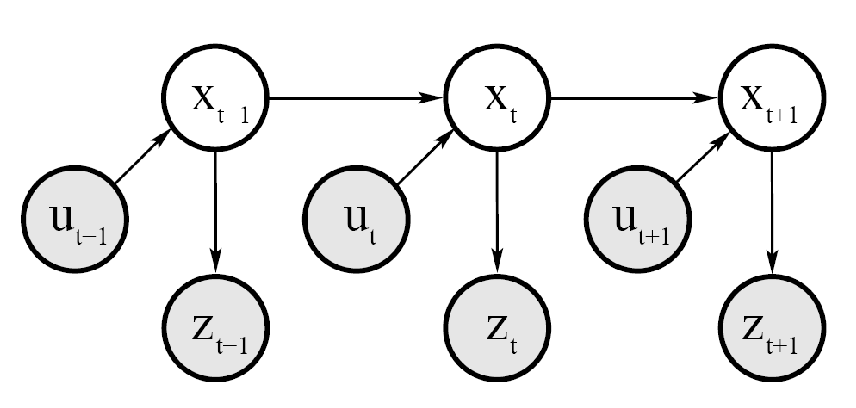
\includegraphics[height = 3.0 in]{../../thesis_work/markov_chain.png}}
  \caption{\label{fig-Markov Chain} A temporal Bayesian model with hidden states $x_{t}$, observations $z_{t}$ and controls $u_{t}$. Figure taken from \cite{thrun2005probabilistic}}
\end{figure}

%\begin{figure}[hbtp]
%\caption{Markov Chain}
%\centering
%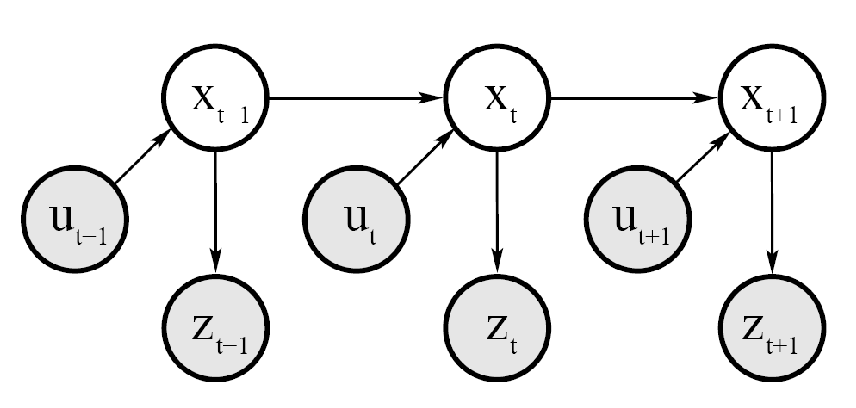
\includegraphics[scale=0.5]{../../thesis_work/markov_chain.png}
%\end{figure}
Thrun \cite{thrun2005probabilistic} stated that the key idea behind particle filter is to represent the posterior bel$(x_{t})$ by a set of random state samples drawn from this posterior. Instead of representing the distribution by a parametric form particle filter represents a distribution by a set of samples drawn from this distribution. In Figure ~\ref{fig: particle representation} the belief is represented by a set of particles. The representation is a approximation but it is nonparametric and therefore there are advantages of using particle filters as an alternative to Extended Kalman Filter and Unscented Kalman Filter. Particle Filters can represent a broader space of distributions for example non-Gaussian and can model non linear transformations of random variables. In Figure ~\ref{fig: particle representation} particle filters are shown to model non-linear transformations. 

The objective of particle filters is to estimate the state of the system given the observation variables. They are designed for Hidden Markov Models(Fig ~\ref{fig-Markov Chain}), where the system consists of hidden and observed variables. In this model the state $x_{t}$ is the hidden random variable as it is not directly observed. The state at time $t$ is only dependent upon the state at time $t-1$ and external influences such as control $u_{t}$. The measurement $z_{t}$ depends on the state at time $t$. The knowledge about the influence of the control on the system can be used to calculate a new expected location and the measurement can be combined in a Bayesian way.


\begin{figure}
\centering
{\includegraphics[height = 3.0 in]{/home/rohan/Documents/thesis_work/particle_filter_non_gaussian_thrun.png}}

\caption{\label{fig: particle representation} The ``particle'' representation used by particle filters. The lower upper right graphs shows samples drawn from a Gaussian random variable, X. These samples are passed through the nonlinear function shown in the upper right graph. The resulting samples are distributed according to the random variable Y. Figure taken from \cite{thrun2005probabilistic}}
\end{figure}

The algorithm for particle filters is described below-:

\begin{algorithm}[H]
\label{alg:ParticleFilter}
 \SetAlgoLined
  		 
 \KwIn{$ X _{t-1}$: particle set \\
 $u_{t}$: most recent control \\
 $z_{t}$: most recent measurement}


 \KwOut{ $X_{t}$:particle set }
\Begin{
\For { m=1 to M do} 
{sample $x_{t}^{m}~p(x_{t}|u_{t},x_{t-1}^m)$
$w_{t}^{m}=p(z_{t}|x_{t}^{m})$
$X_{t}^{-}=X_{t}^{-}+(x_{t}^{m},w_{t}^m)$}

\For{m=1 to M do}
{
draw $i$ with probability $\propto$ $w_{t}^{[i]}$
\\
add $x_{t}^{[i]}$ to $X_{t}$}
return $X_{t}$
}
\caption{Particle Filter Algorithm. Algorithm taken from \cite{thrun2005probabilistic}}
\end{algorithm}

In algorithm ~\ref{alg:ParticleFilter} each particle $x_{t}^{m}$ is instantiation of the state at time $t$.  The first step is to generate a hypothetical state $x_{t}^{m}$ for time $t$ based on previous state $x_{t-1}^{m}$ and control $u_{t}$. The particles are samples from the state transition distribution $p(x_{t}|u_{t},x_{t-1})$. The importance factor for each particle $x_{t}^{m}$ is calculated and denoted by $w_{t}^{m}$. Importance factor is defined as the probability of measurement $z_{t}$ under the particle $x_{t}^{m}$. This probability is defined by a sensor model $p(z_{t}|x_{t})$ Thus importance factor are used to incorporate the measurements into the particle set. In practice, the number of particles used are a large number(e.g.-:1000).

The key part of the algorithm is the re-sampling step in particle filter algorithm. The algorithm draws M particles with replacement from a temporary particle set $X_{t}^{-}$. The probability of drawing the particles is given by the importance factor. The re-sampling step is a probabilistic implementation of the Darwinian idea of survival of the fittest. It refocuses the particle set to regions in state space with high posterior probability. 

Particle Filters is an integral part of my algorithm to learn the right parameters of the motion model and the way it is used is explained in ~\ref{ch:adapting the motion model}.

\section{Particle smoothing}
\label{ch-: particle smoothing}
The particle filter algorithm as described before is the first step in the Expectation process. The next algorithm that completes the Expectation Step is the particle smoothing. Doucet \cite{doucet2009tutorial} in his paper stated that filtering based on observations received up to the current time is used to estimate the distribution of the current state of an Hidden Markov Model (HMM) whereas smoothing is used to estimate distribution of state at a particular time given all the observations up to some later time (Figure ~\ref{fig: particle smoothing}). Russel and Norving \cite{russell2003artificial} showed that the state of the system is better estimated by smoothing as it incorporates more information than just filtering. We use particle smoothing algorithm proposed by Teddy N Yap and Christian R. Shelton \cite{Yap2008} which was based on the technique presented by Docuet et al. \cite{doucet2000monte} and Godsill et al. \cite{Godsill2004}.
\begin{figure}
\centering
{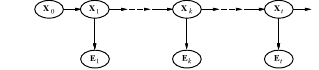
\includegraphics[height = 3.0 in]{/home/rohan/Documents/thesis/smoothing.png}}

\caption{\label{fig: particle smoothing} Smoothing computes $P(X_{k}|e_{1:t})$, the posterior distribution of the state at some past time $k$ given a complete sequence of observations from 1 to $t$. Figure taken from \cite{russell2003artificial}}.
\end{figure}

Particle smoothing is carried out in order to generate samples from the entire joint smoothing density $p(x_{0:T}|u_{1:T},z_{1:T})$. 
The equations described by Yapp \cite{Yap2008} are

\begin{equation}
p(x_{0:T}|u_{1:T},z_{1:T})=\prod_{t=0}^{T}p(x_{t}|x_{t+1:T},u_{1:T},z_{1:T})
\end{equation}

where,

\begin{eqnarray}
p(x_{t}|x_{t+1:T},u_{1:T},z_{1:T}) & = & p(x_{t}|x_{t+1},u_{1:t+1},z_{1:t})\\
 & = & \frac{p(x_{t+1}|x_{t},u_{1:t+1},z_{1:t})p(x_{t}|u_{1:t+1},z_{1:t})}{p(x_{t+1}|u_{1:t+1},z_{1:t})}\\
 & = & \frac{p(x_{t+1}|x_{t},u_{t+1})p(x_{t}|u_{1:t},z_{1:t})}{p(x_{t+1}|u_{1:t+1},z_{1:t})}\\
\label{eq:smoothing_backward} & \alpha & p(x_{t+1}|x_{t},u_{t+1})p(x_{t}|u_{1:t},z_{1:t})
\end{eqnarray}

Equation ~\ref{eq:smoothing_backward} is used to generate states backwards in time give future states. $p(x_{t+1}|x_{t},u_{t+1})$ is the state transition probability and $p(x_{t}|u_{1:t},z_{1:t})$ is obtained by performing particle filtering. 
\begin{comment}
 This technique assumes that particle filtering has been carried out on the data set which results in a set of particles $X_{t}$ with their corresponding weights. The states can be generated recursively backwards in time given the future states using equation ~\ref{eq:smoothing_backward}. $p(x_{t}|u_{1:t},z_{1:t})$ can be obtained by performing particle filtering. $p(x_{t}|x_{t+1:T},u_{1:T},z_{1:T}$ can be approximated by particles with modified importance weights $w_{t|t+1}^{[i]} \alpha w_{t}^{[i]}p(x_{t+1}|x_{t}^{[i]},u_{t+1})$ given filtered particles $x_{t}^{[i]}$.  
\end{comment}




Algorithm ~\ref{alg:Particle Smoothing} shows the step involved to sample from the entire joint smoothing density.

\begin{algorithm}[H]
 \SetAlgoLined
  	\label{alg:Particle Smoothing}
 \KwIn{$ X _{t}, t = 0, 1, ..., T$: particle approximations to the posterior pdfs $p (x _{t}|c _{1:t}, s _{1:t}) , t = 0, 1, ..,T$ 
\\
$c _{1:T} = (c _{1}, c _{2}, ..., c _{T} )$: set of controls from time 1 to time T}
 \KwOut{ $x ^{'} _{0:T} = (x ^{'}_{0},x ^{'}_{1}, ...,x^{'}_{T} )$: a sample from the entire joint smoothing density $p (x_{0:T} |c _{1:T} , s _{1:T} )$ }
\Begin{draw \textit{i} with probability $\propto$ $w ^{[i]} _{T}$
$x ^{'} _{T} \leftarrow x^{[i]}_{T}$
\\
\For {$t \leftarrow T-1$ down to 0 do}{\For{ $i \leftarrow 1 to N_{s}$ do}{$w ^{[i]}_{t|t+1} \leftarrow w ^{[i]} _{t}p(x ^{'} _{t+1}|x_{t}^{[i]},u _{t+1})$}draw \textit{i} with probability $\propto w ^{[i]} _{t|t+1}$\\ $x^{'} \leftarrow x^{[i]}_{t}$}}
	\caption{Sample the entire joint smoothing density $p(x_{0:T}|c_{1:T},s_{1:T})$}
	
\end{algorithm}

In the first step of the algorithm a particle is drawn with probability proportional to the filtered weight of the particles. The next step is to move a time step back and modify the weights of the particles by calculating the new smoothed weights. The new smoothed weights are the product of state transition probability $p(x ^{'} _{t+1}|x_{t}^{[i]},u _{t+1})$ and the weight of the particle $w_{t}^{[i]}$. The next step in the algorithm is to draw particles with probability proportional to new smoothed weights $w_{t|t+1}^{[i]}$.  The sequence of particles $x^{'}$ drawn from joint smoothing density $p(x_{0:T}|c_{1:T},s_{1:T})$ from time 0 to time T form a sampled trajectory $x^{'}_{0:T} \triangleq (x^{'}_0,x^{'}_1,.....,x^{'}_T)$.
 
\chapter{Learning the motion model}
\label{learning the motion model}
\section{Introduction}
\subsection{Work done so far on learning motion model}
The process of calibration has been discussed right from when robotics was introduced and the literature is full of different methods to calibrate a robot (eg-: \cite{cox1990autonomous} \cite{vukobratovic1989introduction}). Virtually all the methods discussed before Roy's work \cite{Roy} required human intervention and assumed the world to be static. These methods required a human to have experience and a device to measure the exact movement of a robot to calibrate. The most important assumption that these methods made was that the physics of a robot never changed and operated in a static environment. 

Roy and Thrun first proposed an online self-calibration method \cite{Roy} in 1999 that adapted to changes that occurred during the lifetime of a robot. The algorithm was designed for land robots where the final pose was given by equations described below

\begin{equation}
x^{'}=x+Dcos(\theta+T)
\end{equation}
\begin{equation}
y^{'}=y+Dsin(\theta+T)
\end{equation}
\begin{equation}
\theta^{'}=(\theta+T)mod2\pi
\end{equation}

$D$ and $T$ are the true translational and rotation of a robot. The measured translational and rotational is $d$ and $t$ and if robot's odometry is accurate then $D=d$ and $T=t$. In practice there is a difference and Roy represents $D$ and $T$ by equations ~\ref{eq-: thrun_noise_D} and ~\ref{eq-: thrun_noise_T} respectively.

\begin{equation}
\label{eq-: thrun_noise_D}
D= d+ \sigma_{trans}d+\epsilon_trans
\end{equation}

\begin{equation}
\label{eq-: thrun_noise_T}
  T= t+ \sigma_{rot}d+\epsilon_{rot}
\end{equation}

$\epsilon_{trans}$ and $\epsilon_{rot}$ are the random variables with zero mean. $\sigma_{trans}$ and $\sigma_{rot}$ are the systematic error, drift.  The algorithm they propose is used to estimate $\sigma_{trans}$ and $\sigma_{rot}$ using sensor data collected throughout robot's motion. They treat the problem as maximum likelihood estimation problem where the parameters are estimated under a dataset $z$ (equations ~\ref{eq-:max_likelihood_thrun}) .

\begin{equation}
\label{eq-:max_likelihood_thrun}
 (\sigma_{trans}^{*},\sigma_{rot}^{*}) = argmax P(\sigma_{trans},\sigma_{rot}|z)
\end{equation}

Austin and Eliazar \cite{Eliazar2004} proposed a different method to achieve the same goals proposed by Roy and Thrun. Their algorithm was different from Roy and Thrun for two reasons. Firstly, Austin ad Eliazar used a more general model which incorporated independence of motion terms. Secondly, the method was able to estimate parameters for non systematic errors as well. 
The motion model proposed by them to account is described below.
\begin{equation}
	\begin{aligned}
	x^{'}&=&x+Dcos(\theta+T/2) \\
	y^{'}&=&y+Dsin(\theta+T/2) \\
	\theta^{'}&=&(\theta+T/2)mod2\pi
	\end{aligned}
\end{equation}
As the turn and drive commands are performed independently therefore to not violate this assumption this model makes T reasonably small and it is absorbed as part of noise. To estimate non-systematic errors the true translational($D$ and rotation($T$) are represented by normal distribution with mean $d$ and $t$ and the variance will scale with $d^2$ and $t^2$ as shown in equation ~\ref{eq-:noise_model_eliazar}
\begin{equation}
\label{eq-:noise_model_eliazar}
\begin{aligned}
D &\sim& \mathcal{{N}}(d\mu_{D_{d}}+t\mu_{D_{t}},d^2\sigma_{D_{d}}^2+t^2\sigma_{D_{t}}^2)\\
T &\sim& \mathcal{{N}}(d\mu_{T_{d}}+t\mu_{T_{t}},d^2\sigma_{T_{d}}^2+t^2\sigma_{T_{t}}^2)
\end{aligned}
\end{equation}

where $\mu_{A_{b}}$ is the coefficient for the contribution of odometry term b to the mean of the distribution over A. The algorithm is used to learn these set of mean and variances.

The method by Austin an Eliazar used Expectation Maximization framework to learn the parameters of the motion model for land robots. In the E step particle filtering and smoothing were performed to get a set of trajectories. In M step the maximum likelihood values of parameters given the trajectories was calculated. Teddy Yapp \cite{Yap2008} used the same framework and learned parameters for motion as well as sensor model of land robots (Figure ~\ref{fig-parameter_estimation Yapp}). They adopted the same motion model but with slightly different noise model as shown in equation ~\ref{eq-:noise_model_yapp}.
\begin{figure}
  \centering
     {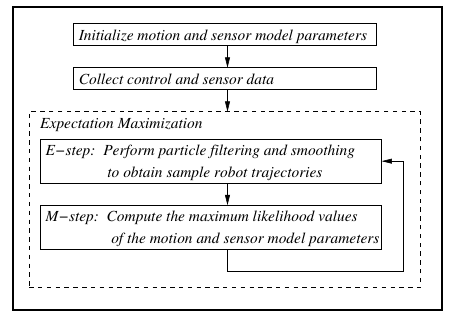
\includegraphics[height = 3.0 in]{/home/rohan/Documents/thesis_work/parameter_estimation_yapp.png}}
  \caption{\label{fig-parameter_estimation Yapp} Block Diagram for the parameter estimation framework. Figure taken from \cite{Yap2008}.}
\end{figure}

\begin{equation}
\label{eq-:noise_model_yapp}
\begin{aligned}
D &\sim& \mathcal{{N}}(d,d^2\sigma_{D_{d}}^2+t^2\sigma_{D_{t}}^2+\sigma_{D_{1}}^2) \\
T &\sim& \mathcal{{N}}(t,sigma_{T_{d}}^2+t^2\sigma_{T_{t}}^2+\sigma_{T-{1}}^2)
\end{aligned}
\end{equation}

The extra constant terms $\sigma_{D_{1}}$ and $\sigma_{T_{1}}$ are added to account for the errors that are not proportional to the translation or rotation of a robot. 

All the work above was done to calibrate our models and Hegrenaes \cite{Hegrenæs2008} in his work showed the importance of motion model for navigation in underwater vehicle. They proposed a novel approach for navigation systems in which knowledge about the vehicle dynamics was used to aid the Inertial Navigation System(INS). The new navigation system was tested on real dataset collected by an AUV.

For navigation in AUV velocity of the vehicle needs to be estimated and sensors such as IMU, DVL etc. are used. In a traditional INS system the key component is an IMU and a set of navigation equations. The reading from accelerometer and gyroscope are integrated to get an estimate of velocity, position and orientation. The reading from such sensors consist of inherent errors and leads to drift in the INS system. Generally sensors such as surface GPS, DVL etc. are an aiding system to the INS (Figure ~\ref{fig-INS systems}(a)). Combination of such systems leads to better estimate of velocity, position and orientation \cite{leonard1998autonomous}. 

Hergreanaes points out an alternative velocity information such as velocity estimate through vehicle dynamics is required because there are situations where it is not possible for the AUV to surface and get a GPS reading or DVL measurement needs to be discarded due to poor quality. The high level system outline for such a model is shown in Figure ~\ref{fig-INS systems}(b).

The system is very similar to traditional INS except that the vehicle model output in also integrated to the system. The vehcile model output doesn't require any extra instruments therefore can be easily applied to any vehicle. An alternative velocity estimate aids the INS where DVL readings are lacking as well as gives redundancy to the system. 




\begin{figure}
  \centering
  \subfigure[Traditional aided INS]{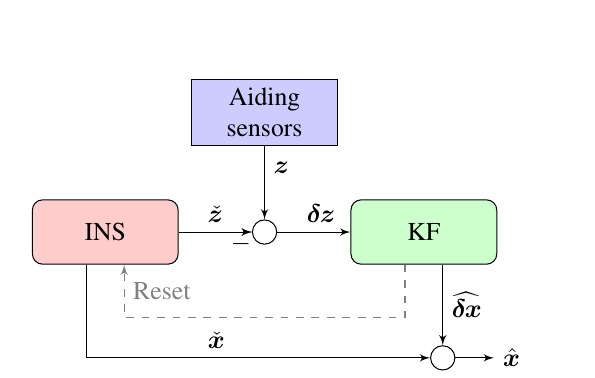
\includegraphics[width = 2.75 in]{/home/rohan/Documents/thesis_work/model_aided_intertial_nvaigation_system_traditional.png}}\qquad
  \subfigure[Model-aided INS]{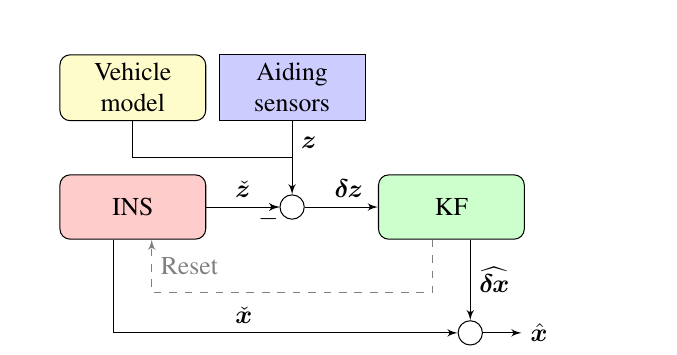
\includegraphics[width = 2.75 in]{/home/rohan/Documents/thesis_work/model_aided_intertial_nvaigation_system_model.png}}
 
  \caption{\label{fig-INS systems}High level system outline. The vehicle model can be used in parallel to external aiding sensors. Figure taken from \cite{Hegrenæs2008}}
\end{figure}

All the above calibration methods are designed for odometric based motion models and for land robots. The use of vehicle model to aid the INS for navigation purposes shows us the importance of an adaptive motion model. The algorithm that I propose is for underwater vehicles and velocity based motion model. The process to adapt the motion model is similar to the previous work by Yapp and Eliazar and our approach is described in rest of the chapters.

\subsection{General Architecture}
In this section we give an overview of the system and point out the differences in my system(Figure ~\ref{fig-General Architecture}) as compared to the existing system proposed by Yapp \cite{Yap2008}. 
\begin{figure}
  \centering
     {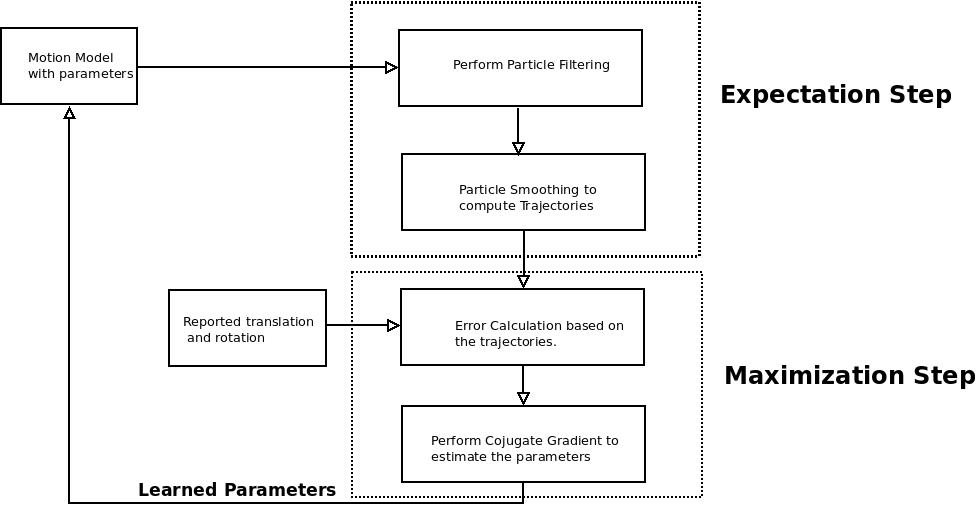
\includegraphics[height = 3.0 in]{Diagram1.jpeg}}
  \caption{\label{fig-General Architecture} Block diagram for the algorithm proposed to adapt motion model.}
\end{figure}
Figure ~\ref{fig-General Architecture} is an outline of the proposed system. The motion and sensor models are initialized with a set of parameters. Given the motion model $p(x_{t}|x_{t-1},u_{t})$, sensor model $p(z_{t}|x_{t})$ and the pose $p(x_{t-1})$ of a robot we can perform particle filtering using Algorithm ~\ref{alg:ParticleFilter}. It is performed to estimate the pose $p(x_{t})$ of a robot at next time step. 

The key ingredient to learn the motion model is to have an estimate of ground truth. To get an idea of ground truth particle smoothing (algorithm ~\ref{alg:Particle Smoothing}) is performed on the particle set produced by particle filtering. The algorithm can be repeated several times to get a set of trajectories. Particle filtering and smoothing are the key algorithm for the Expectation Step. 

The reported translational and rotational movement of a robot is recorded for every time step. Based on the trajectories and reported movements the errors are calculated at each time step. After we have a set of errors we perform Newton Conjugate gradient on the error function to estimate parameters. This completes the Maximization Step.

The learned parameters are reassigned to the motion model and helps in adapting our model to changes in robot and the environment. The whole algorithm is repeated at every time step so that we can dynamically learn the right parameters.

The system proposed for parameter estimation is similar to the system by Yapp \cite{Yap2008}. I use the same EM framework and conjugate gradient to learn the right parameters for the model. The difference lies that the motion model learned is a velocity based motion model as compared to odometry based model. Secondly we focus on underwater environments and therefore use side sonar images to calculate landmarks on the fly for our sensor model as compared to a static map.

\section{Adapting Motion Model}
\label{adapting the motion model}
\subsection{Expectation Maximization}

Expectation Maximization is an iterative process of finding maximum likelihood of parameters of a model which depend upon hidden variables. It is used to estimate unknown parameters $\theta$ given the observed data $X$. A complete dataset can be represented by ${X,Z}$ where $Z$ is a non-observed (hidden, latent) variable. In practice a complete dataset is not given and only a set of observations or incomplete dataset $X$ is found. The hidden variables are important to a problem but complicate the learning process ~\cite{russell2003artificial}. In order to learn with hidden variables Dempster et al. \cite{dempster1977maximum} proposed a method to maximize the probability of the parameters $\theta$ give the dataset $X$ with hidden variables $Z$ called as EM.

\begin{equation}
\label{eq-:em_description}
\theta^{*}=arg max_{\theta} \int p(\theta,Z|X)dZ
\end{equation}

The key idea behind the EM algorithm is to alternate between estimating parameters $\theta$ and hidden variable $Z$.
The E step consists of finding the posterior distribution of hidden variables $p(Z|X,\theta^{old})$ given the current estimate of parameters $\theta^{old}$. The posterior distribution it used to find a expectation of the likelihood of the data for some parameter $\theta$ as shown in equation ~\ref{eq-:maximization}. 
\begin{equation}
\label{eq-:maximization}
\mathcal{Q}(\theta,\theta^{old})=\sum_{Z}p(Z,X|\theta^{old}) \ln p(X,Z|\theta)
\end{equation}
In the M step we maximize the function as shown in  to estimate the new parameters $\theta^{new}$.
\begin{equation}
\theta^{new}=arg max_{theta} \mathcal{Q}(\theta,theta^{old})
\end{equation}

The objective as described by Minka \cite{minka1998expectation} is to maximize $\mathcal{Q}(\theta,\theta^{old})$ and we want an updated estimate of $\theta^{new}$ such that 
\begin{equation}
\theta^{new}>\theta^{old}
\end{equation}
or we want to maximize the difference,
\begin{equation}
\mathcal{Q}(\theta^{new})-\mathcal{Q}(\theta^{old})=\ln P(X|\theta^{new}) - \ln P(X|\theta^{old})
\end{equation}
The above equations with hidden variables can be written as
\begin{equation}
\label{eq-:derivation_em}
\mathcal{Q}(\theta^{new})-\mathcal{Q}(\theta^{old})=\ln(\sum P(X|z,\theta^{new}) P(Z|\theta^{new})) - \ln P(X|\theta^{old})
\end{equation}

Using Jensen's Equality it can be show that,
\begin{equation}
\ln \sum_{i=1}^{n}\lambda_{i}x_{i} \geq \sum_{i=1}^{n}\lambda_{i}\ln(x_{i})
\end{equation}
for constants $\lambda_{i} \geq 0$ with $\sum_{i=1}^{n}\lambda_{i}=1$. This can be applied to equation ~\ref{eq-:derivation_em} and $\lambda=P(Z|X,\theta^{old})$. As $P(Z|X,\theta^{old})$ is a probability measure we have $P(Z|X,\theta^{old}) \geq 0$ and $\sum_{Z}P(Z|X,\theta^{old})=1$.

\begin{eqnarray}
Q(\theta^{new})-Q(\theta^{old}) & = & \ln(\sum_{Z}P(X|Z,\theta^{new})P(Z|\theta))-\ln P(X|\theta^{old})\\
 & = & \ln(\sum_{Z}P(X|Z,\theta^{new})P(Z|\theta).\frac{P(Z|X,\theta^{old})}{P(Z|X,\theta^{old})})-\ln P(X|\theta^{old})\\
 & = & \ln(\sum_{Z}P(z|X,\theta^{old})\frac{P(X|Z,\theta^{new})P(Z|\theta^{new}}{P(Z|X,\theta^{old})})-\ln P(X|\theta^{new})\\
 & \geq & \sum_{Z}P(Z|X,\theta^{old})\ln(\frac{P(X|Z,\theta^{new})P(Z|\theta^{new})}{P(Z|X,\theta^{old})})-\ln P(X|\theta^{old})\\
 & = & \sum_{Z}P(Z|X,\theta^{old})\ln(\frac{P(X|Z,\theta^{new})P(Z|\theta^{new})}{P(Z|X,\theta^{old})P(X|\theta^{old})})\\
 & \triangleq & \triangle(\theta^{new}|\theta^{old})
\end{eqnarray}
We continue by writing

$\mathcal{Q}(\theta^{new})\geq\mathcal{Q}(\theta^{old})+\triangle(\theta^{new}|\theta^{old})$

and for convenience define,

$q(\theta^{new}|\theta^{old})\triangleq\mathcal{Q}(\theta^{old})+\triangle(\theta^{new}|\theta^{old})$

The function $q(\theta^{new}|\theta^{old})$ is bounded by the likelihood
functions $\mathcal{Q}(\theta^{new})$. We need to choose values of
$\theta^{new}$so that $\mathcal{Q}(\theta^{new})$ is maximized.
The new updated value is denoted by $\theta_{n+1}.$
\begin{eqnarray}
\theta_{n+1} & = & argmax_{\theta}\{q(\theta^{new}|\theta^{old})\}\\
 & = & argmax_{\theta}\{\mathcal{Q}(\theta^{old})+\sum_{Z}P(Z|X,\theta^{old})\ln(\frac{P(X|Z,\theta^{new})P(Z|\theta^{new})}{P(Z|X,\theta^{old})P(X|\theta^{old})})\\
 & = & argmax_{\theta}\{\sum_{Z}P(Z|X,\theta^{old})\ln(P(X|Z,\theta^{new})P(Z|\theta^{new})\}\\
 & = & argmax_{\theta}\{\sum_{Z}P(Z|X,\theta^{old})\ln P(X,Z|\theta^{new})\}\\
\end{eqnarray}

We use the EM algorithm as described by Christopher M. Bishop\cite{bishop2006pattern} in his book. The steps taken in EM algorithm are described below -:
\\
1. Have an initial estimate of the parameters $\theta ^{old}$
\\
2. \textbf{E Step:} Evaluate $p(Z|X,\theta^{old})$
\\
3. \textbf{M Step:} Evaluate $\theta ^{new} = arg max _{\theta} L(\theta,\theta^{old})$
\\
\hspace*{20 mm} where 
$L(\theta,\theta^{old})=\Sigma _{Z} p(Z|X,\theta_{old}) \log p(X,Z|\theta)$
\\
4. Check for the convergence of either the log likelihood or the parameter values. If the convergence criterion is not satisfied then let
\\
\hspace*{20 mm} $\theta \leftarrow \theta^{new} $
\\
and return to step 2
\\
There are various convergence techniques that can be applied in step 4. In our algorithm we use Newton Conjugate Gradient to estimate the right parameters. It is important to point that EM algorithm is local optimization technique and there are situations where it can get stuck in local optimum. 		


\subsection{Parameter Estimation}
\label{ch:adapting the motion model}
In this section we give a detailed explanation of the method proposed to learn motion model. As stated in Chapter ~\ref{chap-:Motion Model} to calculate the position of AUV we need to estimate velocity and feed it to the navigation equation ~\ref{eq-: navigation equation for AUV}. As we are operating in a dynamic environment there are various factors that can lead to changes in our motion model. To adapt the motion model we represent the velocity as a Gaussian distribution. We assume the distribution to be Gaussian as sum of several random noises leads to a such a distribution.   The algorithm described here is used to estimate parameters of the distribution. Another assumption for the algorithm that we represent the pose of an AUV in two dimension as compared to six. 

The velocity based motion model equations used in the algorithm are 

\begin{equation}
 x_{t}=x_{t-1}+V_{t-1}/W_{t-1} \sin(\theta_{t-1})+ V_{t-1}/W_{t-1} \cos(\theta_{t-1} + W_{t-1} \delta t)
\end{equation}

\begin{equation}
\label{eq:velocity motion model_y}
y_{t}=y_{t-1}+V_{t-1}/W_{t-1} \cos(\theta_{t-1})- V_{t-1}/W_{t-1} \sin(\theta_{t-1} + W_{t-1} \delta t)
\end{equation}

\begin{equation}
\label{eq:velocity motion model_theta}
\theta_{t}=\theta_{t-1}+ W_{t-1} \delta t
\end{equation}

where,
\begin{equation}
V \sim \mathcal{N}(v_{t},v_{t}^{2}\sigma_{V_{v}}^{2}+w_{t}^{2}\sigma_{V_{w}}^{2}+\sigma_{V_{1}}^{2})
W \sim \mathcal{N}(w_{t},v_{t}^{2}\sigma_{W_{v}}^{2}+w_{t}^{2}\sigma_{W_{w}}^{2}+\sigma_{W_{1}}^{2})
\end{equation}


The translational and rotational velocity are represented by a Gaussian distribution with mean as reported translational $v$ and rotational $t$ velocity respectively. $\sigma_{A_{b}}$ represents the contribution of the velocity term b to the variance of the distribution over A. $\sigma_{V_{1}} $ and $\sigma_{w_{1}}$ are added to the motion model to account for errors that are not directly proportional to the translation and rotation of a robot.

Putting the whole problem of estimating parameters in EM framework, we define the parameters of the motion model that we want to learn are
$\theta={\sigma_{V_{v}}^{2},\sigma_{V_{w}}^{2},\sigma_{V_{1}}^{2},\sigma_{W_{v}}^{2},\sigma_{W_{t}}^{2},\sigma_{W_{1}}^{2}}$
The data Z from which the parameters can be learned is defined as $Z={u_{1:T},z_{1:T}}$
where, $u_{1:T}$ and $z_{1:T}$ are the history of control and sensor readings. The robot's trajectory is the hidden variable in the system as it not directly observable and can be defined as $r=x_{0:T}$.

The first step in an EM algorithm is to initialize the set of parameters $\theta$ with some initial values. In the E step we calculate the expectation of $\log p(r,Z|\theta)$ with respect to distribution $p(r|Z,\theta)$. The distribution can be also be represented by the entire join smoothing density $p(x_{0:T}|u_{1:T},z_{1:T})$. To approximate the E step i.e. the joint smoothing density, particle filtering and smoothing is performed to calculate a set of robot trajectories as discussed in section ~\ref{ch-: particle smoothing}. In the M step we treat the set of trajectories as ground truth as use them to compute the maximum likelihood of parameters. The algorithm keeps on alternating between the E and M step until convergence. 

For calculating the maximum likelihood values for parameters we need to calculate the motion errors $\epsilon_{T_{t}},\epsilon_{D_{t}}$ based on robot trajectory and the contribution of translational $v$ and rotational $t$ velocity to the errors.

\begin{eqnarray}
\epsilon_{T_{t}}^{[j]}&=&(\theta_{t_{+1}}^{'[j]}-\theta_{t}^{'[j]}-r_{t}^{''})mod2\pi\\
\epsilon_{D_{t}}^{[j]}&=&(x_{t+1}^{'[j]}-x_{t}^{'[j]})cos(\theta_{t}^{'[j]}+\frac{r_{t}^{''}+\epsilon_{T_{t}}^{[j]}}{2}+(y_{t+1}^{'[j]}-y_{t}^{'[j]})sin(\theta_{t}^{'[j]}+\frac{r_{t}^{''}+\epsilon_{T_{t}}^{[j]}}{2})-d_{t}^{''}
\end{eqnarray}

The distribution that represents these errors are 
\begin{eqnarray}
\epsilon_{V_{t}}^{[j]}&\sim&\mathcal{{N}}(0,v_{t}^{2}\sigma_{V_{v}}^{2}+w_{t}^{2}\sigma_{V_{w}}^{2}+\sigma_{V_{1}}^{2})\\
\epsilon_{W_{t}}^{[j]}&\sim&\mathcal{{N}}(0,v_{t}^{2}\sigma_{w_{v}}^{2}+w_{t}^{2}\sigma_{V_{w}}^{2}+\sigma_{W_{1}}^{2})
\end{eqnarray}

where j stands for sampled trajectory.

The likelihood functions are 
\begin{eqnarray}
\mathcal{Q}_{\epsilon_{D}}(\sigma_{V_{v}}^{2},\sigma_{V_{r}}^{2},\sigma_{V_{1}}^{2}) & = & p(\{\epsilon_{V_{v}}^{[j]}\}|u_{1:T},\{k_{0:T}^{[j]}\})\\
 & = & \prod_{j}\prod_{t=0}^{T-1}\frac{1}{\sqrt{2\pi(v_{t}^{2}\sigma_{V_{v}}^{2}+r_{t}^{2}\sigma_{V_{r}}^{2}+\sigma_{V_{1}}^{2})}}*\exp(\frac{(\epsilon_{V_{t}}^{[j]})^{2}}{2(d_{t}^{2}\sigma_{V_{v}}^{2}+r_{t}^{2}\sigma_{V_{r}}^{2}+\sigma_{V_{1}}^{2})}
\end{eqnarray}



\begin{eqnarray*}
\mathcal{Q}_{\epsilon_{T}}(\sigma_{W_{d}}^{2},\sigma_{W_{r}}^{2},\sigma_{W_{1}}^{2}) & = & p(\{\epsilon_{W_{t}}^{[j]}\}|u_{1:T},\{k_{0:T}^{[j]}\})\\
 & = & \prod_{j}\prod_{t=0}^{T-1}\frac{1}{\sqrt{2\pi(v_{t}^{2}\sigma_{W_{d}}^{2}+r_{t}^{2}\sigma_{W_{r}}^{2}+\sigma_{W_{1}}^{2})}}*\exp(\frac{(\epsilon_{W_{t}}^{[j]})^{2}}{2(v_{t}^{2}\sigma_{W_{d}}^{2}+r_{t}^{2}\sigma_{W_{r}}^{2}+\sigma_{W_{1}}^{2})})
\end{eqnarray*}


The estimate the parameters we get the maximum likelihood estimates 

\begin{eqnarray}
\sigma_{V_{v}}^{2*},\sigma_{V_{r}}^{2*},\sigma_{V_{1}}^{2*} & = & argmax_{\sigma_{V_{v}}^{2},\sigma_{V_{r}}^{2},\sigma_{V_{1}}^{2}}\mathcal{Q}(\sigma_{V_{v}}^{2},\sigma_{V_{r}}^{2},\sigma_{V_{1}}^{2})\\
\sigma_{W_{d}}^{2*},\sigma_{W_{r}}^{2*},\sigma_{W_{1}}^{2*} & = & argmax_{\sigma_{W_{d}}^{2},\sigma_{W_{r}}^{2},\sigma_{W_{1}}^{2}}\mathcal{Q}(\sigma_{W_{d}}^{2},\sigma_{W_{r}}^{2},\sigma_{W_{1}}^{2})
\end{eqnarray}

We maximize the log likelihood function via Newton conjugate gradient method with respect to motion model parameters. Conjugate gradient is a method to determine the minimum or maximum of a function \cite{shewchuk1994introduction}. Generally it requires the gradient of the function. In this method the gradient of the function is taken as the first search direction while the next search direction are chosen in such a way that they are orthogonal to all previous search directions. The gradient of log likelihood functions are 

\begin{eqnarray}
\mathcal{{L}}(\sigma_{V_{v}}^{2},\sigma_{V_{w}}^{2},\sigma_{V_{1}}^{2})&=&-\frac{1}{2}\sum_{j}\sum_{t=0}^{T-1}[\log2\pi+\log(v_{t}^{2}\sigma_{V_{v}}^{2}+w_{t}^{2}\sigma_{V_{w}}^{2}+\sigma_{V_{1}}^{2})+\frac{(\epsilon_{V_{t}}^{[j]})^{2}}{v_{t}^{2}\sigma_{V_{v}}^{2}+w_{t}^{2}\sigma_{V_{r}}^{2}+\sigma_{V_{1}}^{2}}\\
\mathcal{{L}}(\sigma_{W_{v}}^{2},\sigma_{W_{w}}^{2},\sigma_{W_{1}}^{2})&=&-\frac{1}{2}\sum_{j}\sum_{t=0}^{T-1}[\log2\pi+\log(v_{t}^{2}\sigma_{W_{v}}^{2}+w_{t}^{2}\sigma_{W_{w}}^{2}+\sigma_{W_{1}}^{2})+\frac{(\epsilon_{W_{t}}^{[j]})^{2}}{v_{t}^{''2}\sigma_{W_{v}}^{2}+w_{t}^{''2}\sigma_{W_{w}}^{2}+\sigma_{W_{1}}^{2}}
\end{eqnarray}
 



\begin{comment}
\section{Application}
In this chapter we describe a specific application for learned motion model in underwater vehicles. A typical navigation sensor system would consists of Inertial Navigation Systems(INS) and some standard compass and pressure sensor. In some of the systems we could have position updates from long baseline(LBL),ultra short baseline(USBL) acoustics and surface GPS. Some high end systems would have Doppler Velocity Log(DVL) which estimates speed over ground or water. These systems are sometimes incorporated to limit the drift of Inertial Navigation System[refer the paper]. Even when a DVL is included there are situations in which DVL fails or the reading have to be discarded due to poor quality. 

We need some sort of alternative velocity information that doesn't depend upon external sensors in order to compensate for the drift in INS. To get an estimate of velocity we can use the kinetic vehicle model to aid the INS. 
\begin{figure}[hbtp]
\caption{Traditional aided INS}
\centering
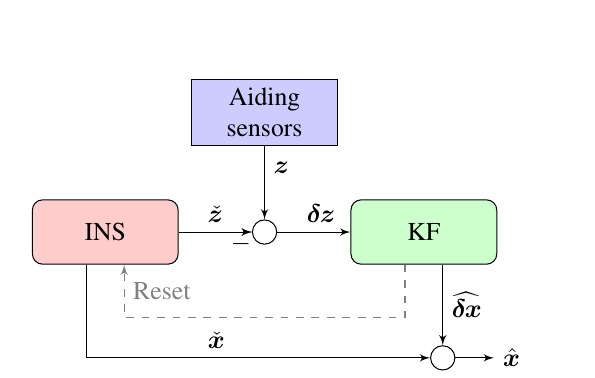
\includegraphics[scale=1.0]{/home/rohan/Documents/thesis_work/model_aided_intertial_nvaigation_system_traditional.png}
\end{figure}

\begin{figure}[hbtp]
\caption{Traditional aided INS}
\centering
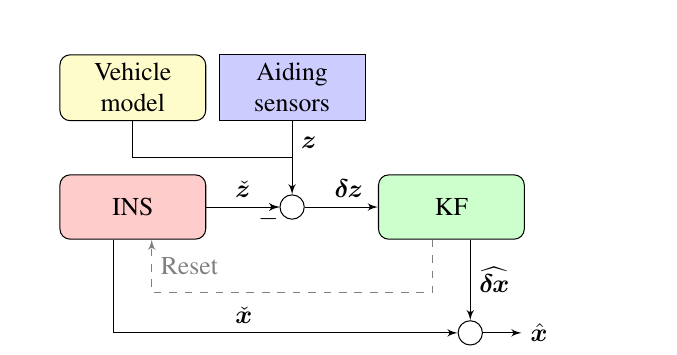
\includegraphics[scale=1.0]{/home/rohan/Documents/thesis_work/model_aided_intertial_nvaigation_system_model.png}
\end{figure}
In the traditional aided INS the readings from gyro and accelerometer measurements from the IMU are integrated over time to give an estimate of velocity,position and orientation. Due to the inherent errors in the gyros and accelerometers there is a drift in  the INS system. There are aiding sensors such as DVL and surface GPS to compensate the drift for the IMU. The reading from the sensors are fused using a Bayes filters to get an enchained estimate of velocity ,position and orientation. 

In the model aided INS the IMU suffers from the same drift but the output from the model is treated analogously to that of an external aiding sensor. In this system the DVL in traditional INS systems are replaced by vehicle model. The output from the model i.e. the velocity estimate is fused with the readings from the INS by a Bayes filter. The integrating of vehicle model with the IMU systems help in systems which lack external velocity measurements. The other implication is in systems where redundancy and integrity is important e.g. during sensor drop outs or sensor failures.

This specific application shows the importance of having a accurate motion model. As stated in earlier chapters the motion model can change due to various factors and would have a direct impact on the navigation systems of underwater vehicles.Wrong estimates from the motion model will not benefit INS systems and overall lead to wrong estimate about the position and orientation of the vehicle. Our algorithm shows on how to learn the motion model on the fly which can lead to better estimate of the velocity and therefore accurate navigation systems.

As you can see in the figure the input to the motion model is a control command and output is the velocity estimate. In HUGIN 4500 they had implemented a static motion model as table look up based on experimental data i.e.
$u_{r}=f(n_{s})$  where $n_{s}$ is the control system set point. The velocity estimate $u_{r}$ is fused with the reading from IMU to get a better estimate of the position of the AUV. As shown before we try to learn the motion model to find the best estimate for the velocity so that it can aid the INS in this particular application. 
\end{comment}

 


\chapter{Results and Experimental Setup}
\label{ch-: results adapting motion model}
In this chapter we describe the experimental setup of the simulator to test our algorithm. To demonstrate the effectiveness of our approach the results from the simulated experiment are also shown.
\section{Experimental Setup}
To test our algorithm for learning the motion model we create a simulated world(Figure ~\ref{fig-: simulation world}). The world size of our simulation is 400X400 with four landmarks shown in blue dots. The red * shows the location of the robot and blue triangle is the location estimate of the  robot by particle filters. The robot is moving with a constant forward and rotational velocity throughout the experiment. In simulation the robot can measure its distance from all four landmarks at all time. The sensor noise in the simulation can be varied in between the experiment. The particle size is 500 and is constant throughout the experiment. Table ~\ref{tab-constant parameters} shows the summary of variables for the experiment to test the effectiveness of our algorithm to learn a motion model.
\begin{table}[tbh]
\centering
\begin{tabular}{|r|r|}
    \hline
    & Experiment \\
    \hline \hline
    World Size & 400 units X 400 units\\
    \hline
    Total timesteps & 200  \\
    \hline
    No. of sensor readings & 200 \\
    \hline
    Translational Velocity & 3 units/timestep \\
    \hline
    Rotational Velocity & 01. units/timestep \\
    \hline
\end{tabular}
 \caption{\label{tab-constant parameters}Summary of the experiments performed to adapt motion model.}
\end{table}

\begin{figure}
  \centering
     {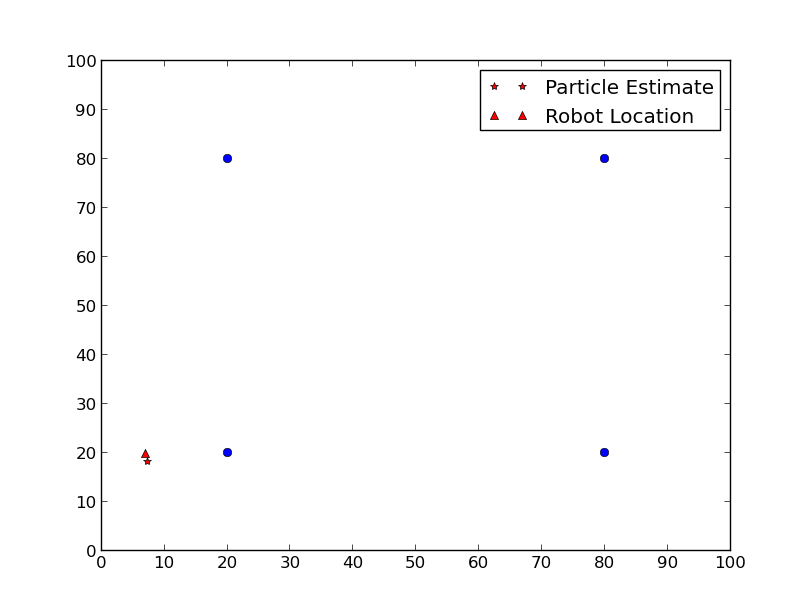
\includegraphics[height = 3.0 in]{0.png}}
  \caption{\label{fig-: simulation world}The simulation environment consisting of the robot(triangle) and the particle estimate of the location(star). The blue dots represent the landmarks.}
\end{figure}


At the start of the experiment  the initial location of the robot and particle filters are randomly initialized (Figure ~\ref{fig-: movement simulation world}(a)). The robot is moved by a constant velocity and Figure ~\ref{fig-: movement simulation world}(b)(c)(d) shows the updated location of the robot as well as an estimate by particle filters of the robot's location.



\begin{figure}
  \centering
  \subfigure[]{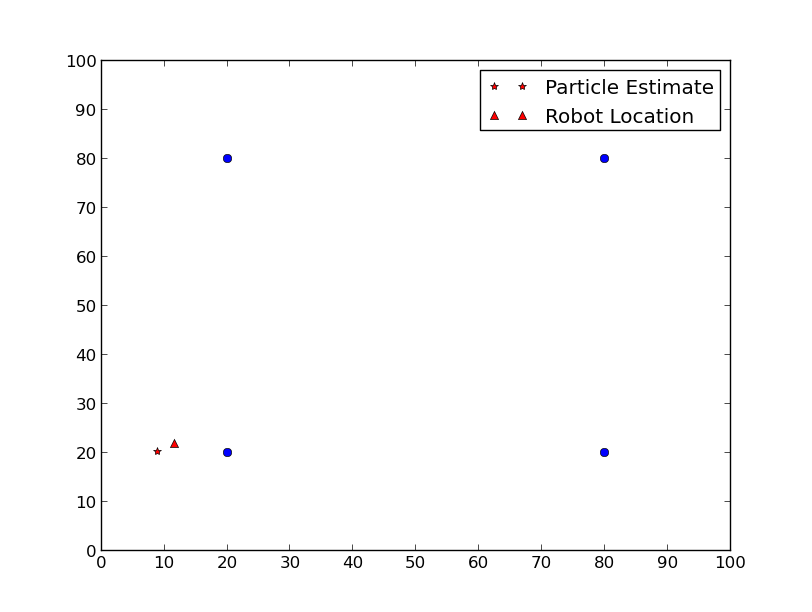
\includegraphics[width = 2.75 in]{1.png}}\qquad
  \subfigure[]{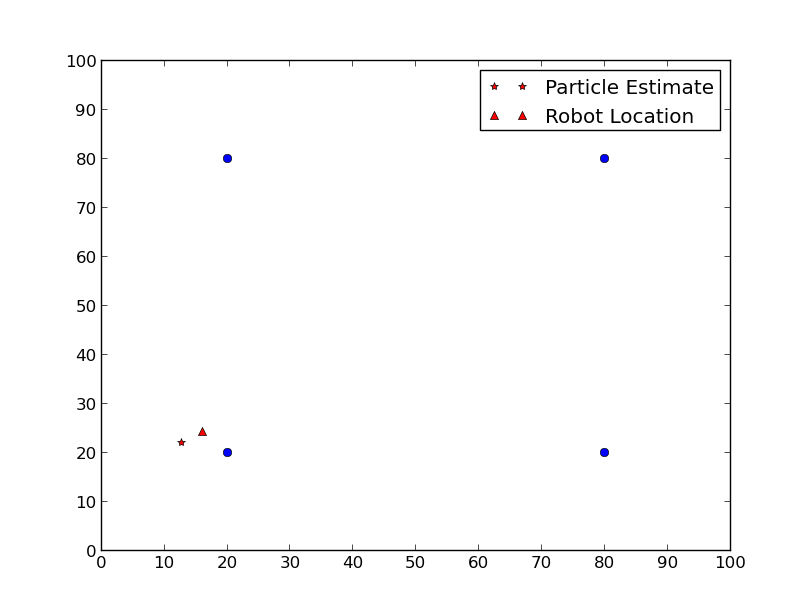
\includegraphics[width = 2.75 in]{2.png}}\qquad
  \subfigure[]{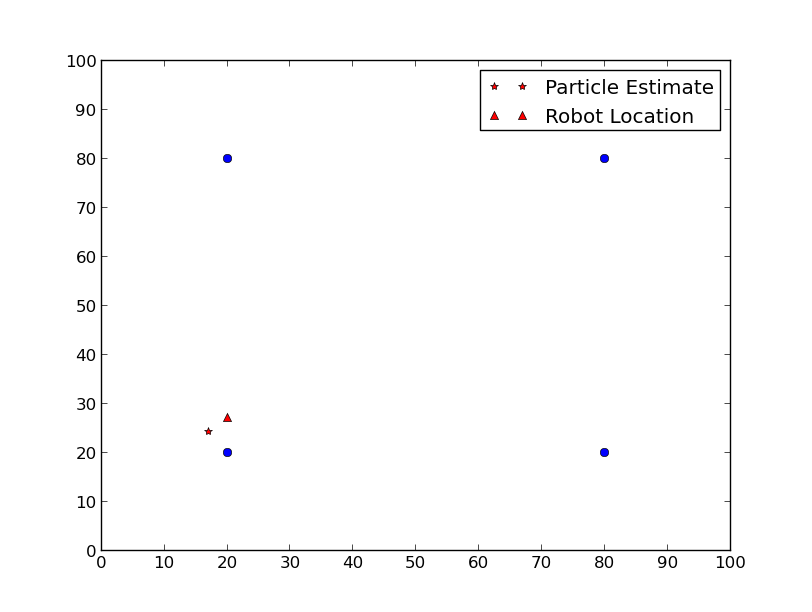
\includegraphics[width = 2.75 in]{3.png}}\qquad
  \subfigure[]{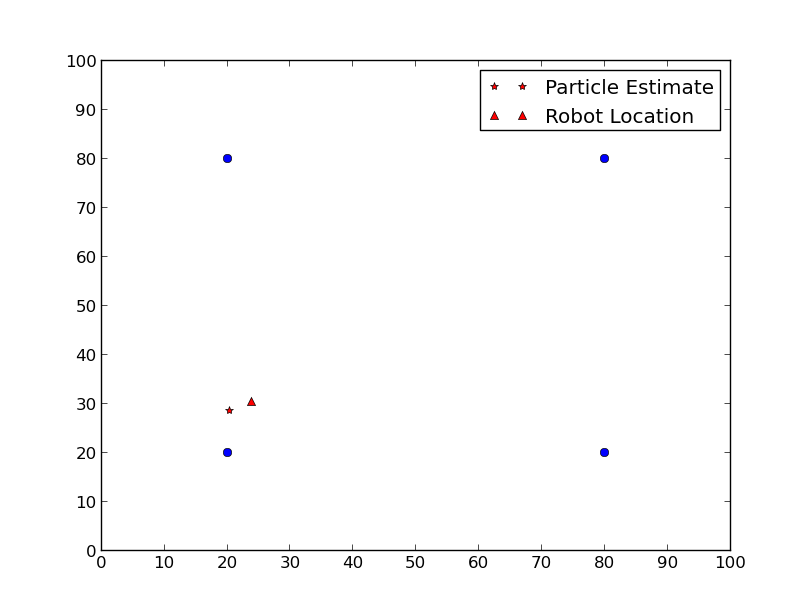
\includegraphics[width = 2.75 in]{4.png}}
  \caption{\label{fig-: movement simulation world}Particle Filters estimating the position of the robot. The robot is moved at a constant velocity of 5 units/timestep in each case. The particle filters estimate the location of the robot (star) by integrating the motion and sensor models.}
\end{figure}



\section{Results}
In this section we describe the various experiments that were performed in our simulated world. To simulate changes in the environment I externally change the noise in robot's motion model. In the experiments external changes were simulated by artificially introducing a drift in the motion. Secondly, by changing the variance of the motion model distribution. As shown in Table ~\ref{tab-constant parameters} the total timesteps is 200 and in all the experiments we simulate the changes at time step 60. 

As described in Chapter ~\ref{chap-:Motion Model} the noise model for our simulated experiment is 

$V_{t}\sim\mathcal{{N}}(v_{t},v_{t}^{2}\sigma_{V_{v}}^{2}+w_{t}^{2}\sigma_{V_{w}}^{2}+\sigma_{V_{1}}^{2})$

$W_{t}\sim\mathcal{{N}}(w_{t},v_{t}^{2}\sigma_{w_{v}}^{2}+w_{t}^{2}\sigma_{V_{w}}^{2}+\sigma_{W_{1}}^{2})$

In first experiment we change $\sigma_{V_{v}}^2$ at time step 60 as shown in Table ~\ref{tab-:varying_sensor_noise}. The changed values of the parameter for first and second case are $0.5$ and $1.0$ respectively. The number of trajectories is 3 and is kept constant for both the cases. In this experiment we keep the sensor noise constant as well. 

\begin{table}[tbh]

\centering



\begin{tabular}{|c|c|c|c|c|c|>{\centering}p{2cm}|>{\centering}p{2cm}|}
\hline 
\multicolumn{2}{|>{\centering}p{2cm}|}{Initial Parameter Values} & \multicolumn{2}{>{\centering}p{2cm}|}{Changed Parameter Values (after 60)} & \multicolumn{2}{>{\centering}p{2cm}|}{Estimated Parameter Values} & Sensor Noise & Trajectories\tabularnewline
\hline
 &  & 1 & 2 & 1 & 2 &  & \tabularnewline
\hline 
$\sigma_{V_{v}}^{2}$ & 0.05 & 0.5 & 1.0 & 0.707 & 1.868 & 1.0 & 3\tabularnewline
\hline 
$\sigma_{V_{w}}^{2}$ & 0.05 & 0.05 & 0.05 & 0.05 & 0.05 & 1.0 & 3\tabularnewline
\hline 
$\sigma_{V_{1}}^{2}$ & 0.05 & 0.05 & 0.05 & 0.123 & 0.252 & 1.0 & 3\tabularnewline
\hline 
$\sigma_{W_{v}}^{2}$ & 0.05 & 0.05 & 0.05 & 1.476 & 1.496 & 1.0 & 3\tabularnewline
\hline 
$\sigma_{W_{w}}^{2}$ & 0.05 & 0.05 & 0.05 & 0.05 & 0.05 & 1.0 & 3\tabularnewline
\hline 
$\sigma_{W_{1}}^{2}$ & 0.05 & 0.05 & 0.05 & 0.208 & 0.210 & 1.0 & 3\tabularnewline
\hline 
\end{tabular}
\caption{\label{tab-:varying_sensor_noise}Initial and estimated values of parameters with constant sensor noise
and trajectories}
\end{table}

As shown in Table ~\ref{tab-:varying_sensor_noise} the estimated value of $\sigma_{V_{v}}^2$ are $0.707$ and $1.868$ which are greater than the actual values and could lead to better localization. In order to demonstrate that I plot the localization error i.e. euclidean error between the robot's actual position and location estimate of particle filters with time. In Figure ~\ref{fig-varying_sensor_noise} the red and blue line shows the error with a static motion model and adaptive motion model respectively.

 
 
\begin{figure}
  \centering
     {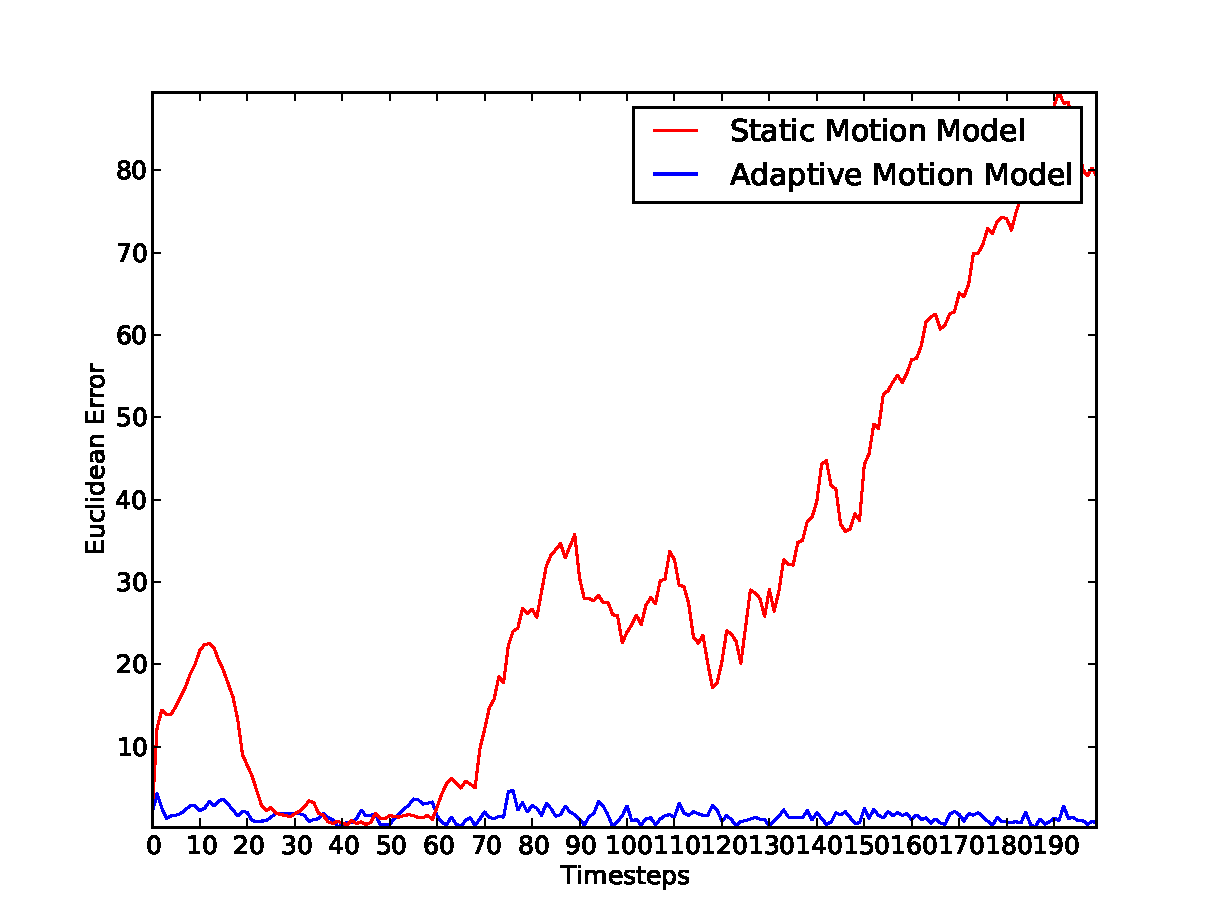
\includegraphics[height = 3.0 in]{./plots/200_005_05_s_10.pdf}}
  \caption{\label{fig-varying_sensor_noise}Plot showing the localization error between robot and the estimate of the robot's location by particle filters. The $\sigma_{V_{v}}^{2}$ is changed from 0.05 to 0.5 at timestep 60. The sensor noise is 1.0}
\end{figure}
At the start of the experiment the parameter values for the robot's motion model and static motion model for particle filters are initialized with the same value. The adaptive motion model right from time step 0 starts estimating the parameters. In Figure ~\ref{fig-varying_sensor_noise} in the first $20$ there is no change and we can see that the adaptive motion model performs better than the static. In theory the static motion model has the best estimate of robot' motion as they are initialized with the same parameter value so the error should be less for static motion model. We don't see this because the location of particles are randomly initialized therefore it might be at different location to robot's start position. It needs sensor model to decrease the error and as the sensor noise is high it takes time to build the weight of particles. In Figure ~\ref{fig-varying_sensor_noise_sensor_model_max_weight} we plot the difference between the maximum weight and average weight of the particle set at each time step. This gives us a measure of distribution of the particle set. If we have a higher difference it means that the particle set contains particle which are sure about robot's location or vice versa. When the weights of particle are higher we can see the 
static motion model performing better. This is due to the resampling step of particle filters where they choose the most probable particles based on motion and sensor models. As soon as the algorithm starts picking the most probable particles the error goes down and we can see that the average weight of particles are also higher. In the case of adaptive motion model the distribution of motion model gets wider right from the start and which leads to decrease in error.

After time step 60 we change the motion model noise and we can see that adaptive motion model performing way better as compared to the static motion model. The difference in the weights of particles in Figure ~\ref{fig-varying_sensor_noise_sensor_model_max_weight} also goes down. In Figure ~\ref{fig-varying_sensor_noise_motion_model} we don't see a jump in the red line or green line at time step 60 and this due to the fact that the estimate of parameter before the change was greater than the change after time step 60. 

   
\begin{figure}
  \centering
     {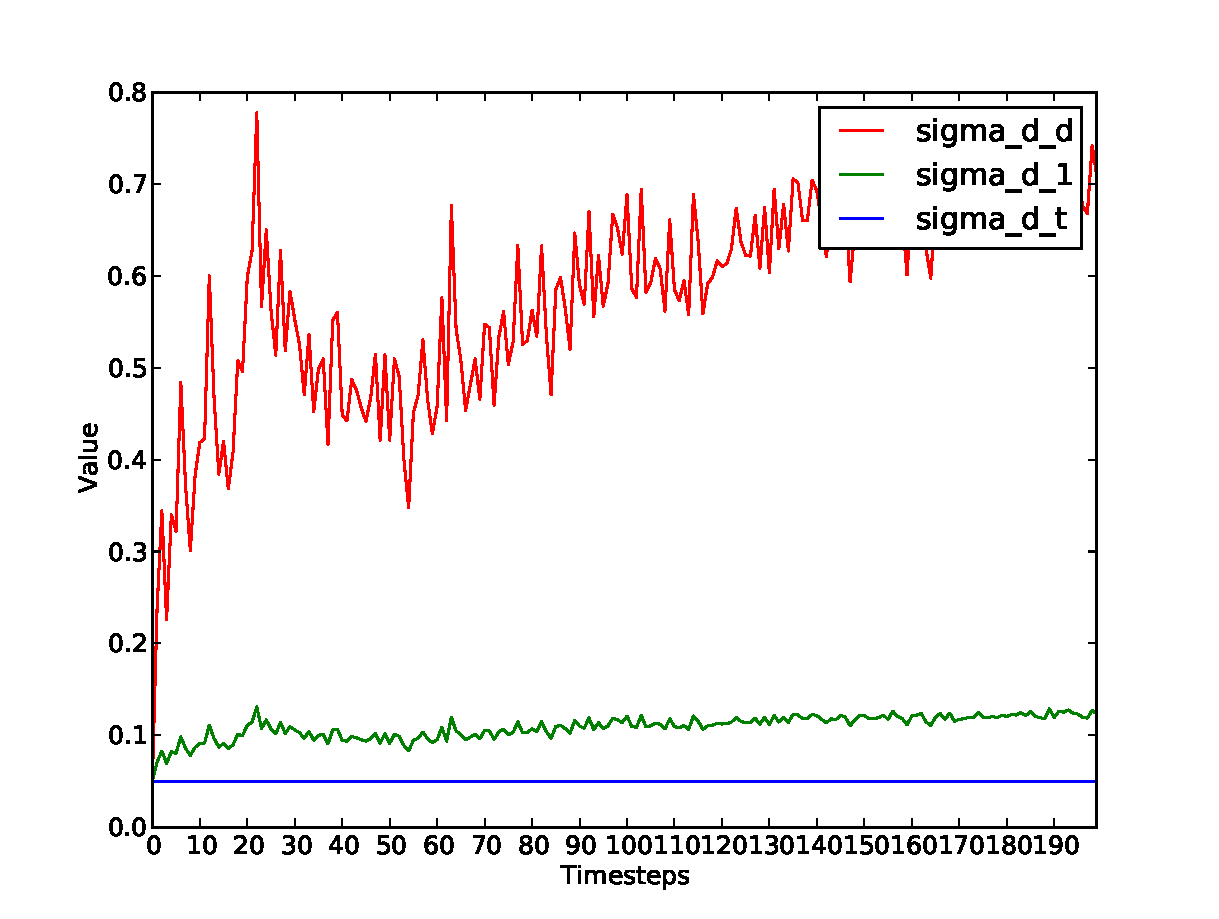
\includegraphics[height = 3.0 in]{./plots/200_005_05_s_10_motion_model_trans.pdf}}
  \caption{\label{fig-varying_sensor_noise_motion_model} Estimate of parameter values $\sigma_{V_{v}}^{2}$, $\sigma_{V_{w}}^{2}$,  $\sigma_{V_{1}}^{2}$ at every time step. The motion model noise $\sigma_{V_{v}}^{2}$ is changed from 0.05 to 0.5 at timestep 60. The sensor noise is 1.0}
\end{figure}

\begin{figure}
  \centering
     {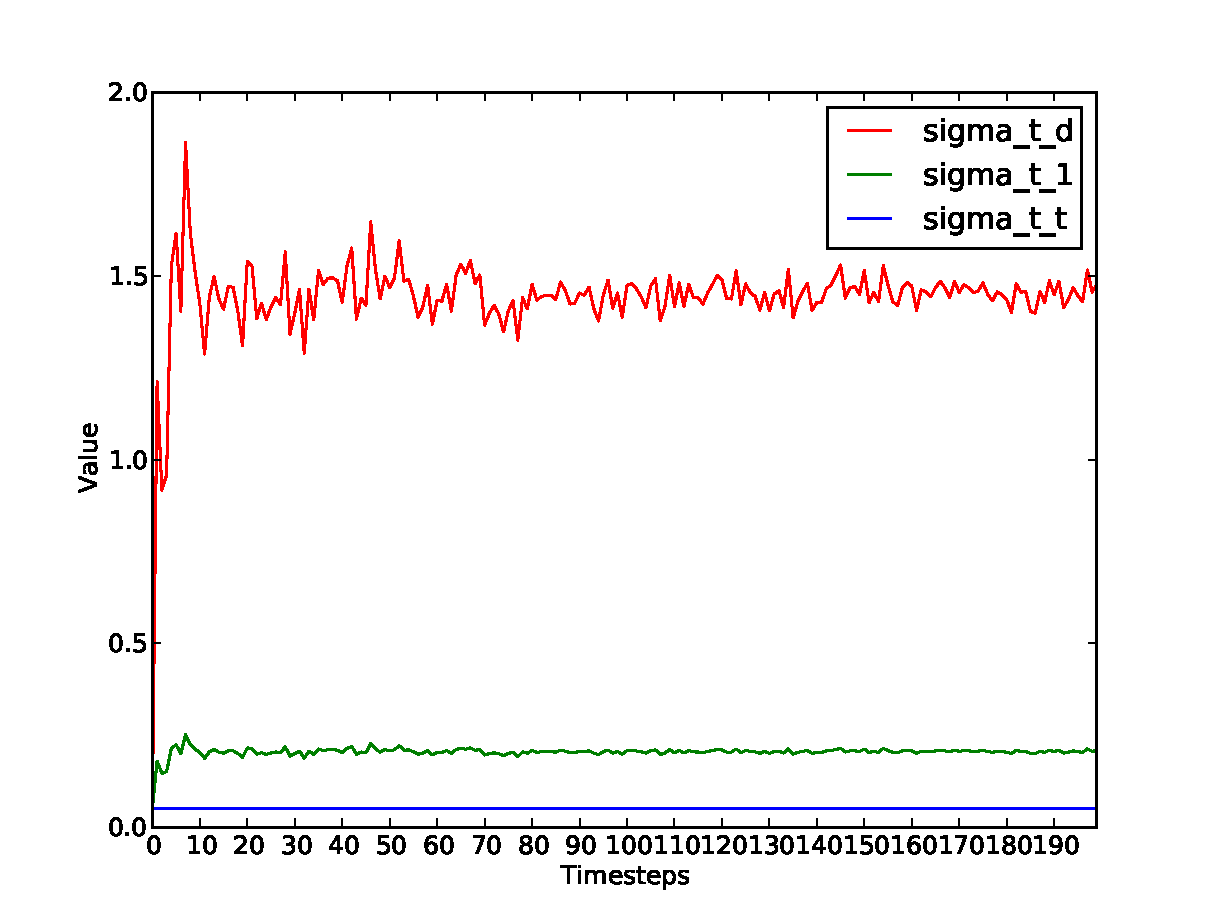
\includegraphics[height = 3.0 in]{./plots/200_005_05_s_10_motion_model_rotation.pdf}}
  \caption{\label{fig-varying_sensor_noise_motion_model_rotation} Estimate of parameter values $\sigma_{W_{v}}^{2}$, $\sigma_{W_{w}}^{2}$, $\sigma_{W_{1}}^{2}$ at every time step. The motion model noise $\sigma_{V_{v}}^{2}$ is changed from 0.05 to 0.5 at timestep 60. The sensor noise is 1.0}
\end{figure}

\begin{figure}
  \centering
     {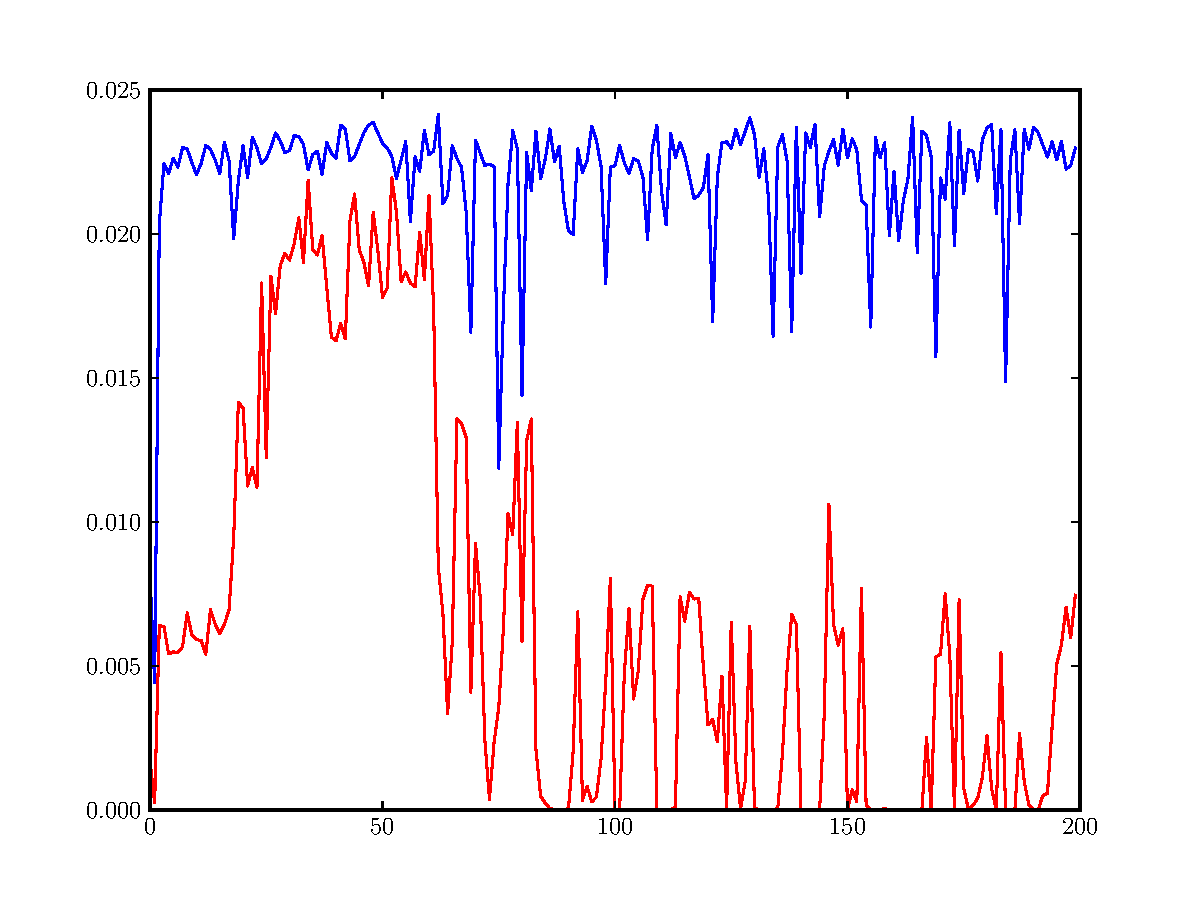
\includegraphics[height = 3.0 in]{./plots/200_005_05_s_10_max_weight.pdf}}
  \caption{\label{fig-varying_sensor_noise_sensor_model_max_weight} Difference between the maximum weight and average weight of the particle set. The motion model noise $\sigma_{V_{v}}^{2}$ is changed from 0.05 to 0.5 at timestep 60. The sensor noise is 1.0 }
\end{figure}

In the next experiment $\sigma_{V_{v}}^2$ is changed from $0.05$ to $1.0$ and the errors, estimation of parameters and average weight are shown in Figure ~\ref{fig-varying_sensor_noise_1.0}, Figure ~\ref{fig-varying_sensor_noise_motion_model_1.0} and Figure \ref{fig-varying_sensor_noise_sensor_model_1.0_max_weight} respectively. 

In both the experiment's the robot's $\sigma_{V_{1}}^2$ is $0.05$ and is not changed throughout the experiment. Table ~\ref{tab-:varying_sensor_noise} shows that in adaptive motion model the estimated value of $\sigma_{V_{1}}^2$ changes from the initialization value. Similarly other parameters such as $\sigma_{W_{V}}^2$ and $\sigma_{W_{1}}^2$ are also changed. This error in estimation is not of much concern as the main goal of the algorithm proposed was to learn the motion model to decrease the localization error. 

\begin{figure}
  \centering
     {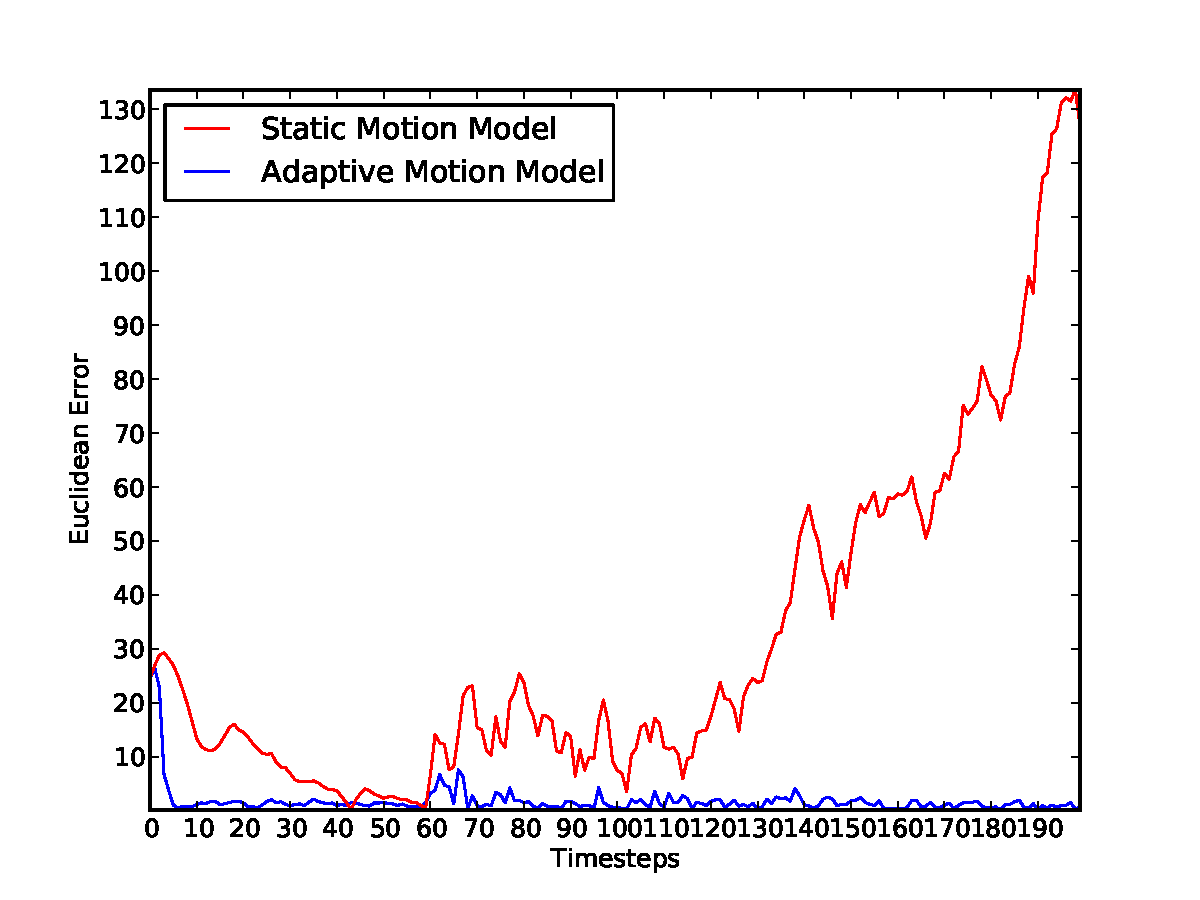
\includegraphics[height = 3.0 in]{./plots/200_005_10_s_10.pdf}}
  \caption{\label{fig-varying_sensor_noise_1.0} Plot showing the localization error between robot and the estimate of the robot's location by particle filters. The $\sigma_{V_{v}}^{2}$ is changed from 0.05 to 1.0 at timestep 60. The sensor noise is 1.0}
\end{figure}
   
   
\begin{figure}
  \centering
     {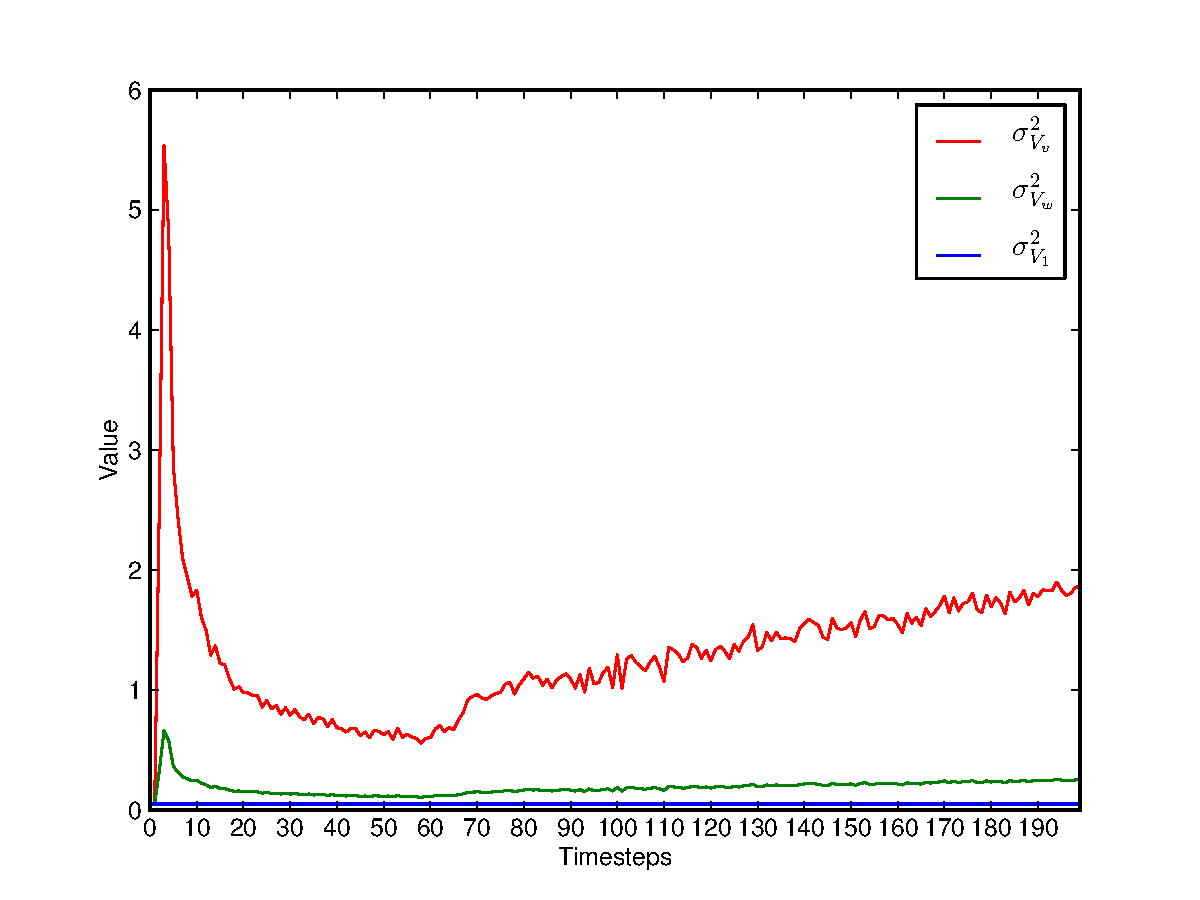
\includegraphics[height = 3.0 in]{./plots/200_005_10_s_10_motion_model_trans.pdf}}
  \caption{\label{fig-varying_sensor_noise_motion_model_1.0}Estimate of parameter values $\sigma_{V_{v}}^{2}$, $\sigma_{V_{w}}^{2}$,  $\sigma_{V_{1}}^{2}$ at every time step. The motion model noise $\sigma_{V_{v}}^{2}$ is changed from 0.05 to 1.0 at timestep 60. The sensor noise is 1.0.}
\end{figure}

\begin{figure}
  \centering
     {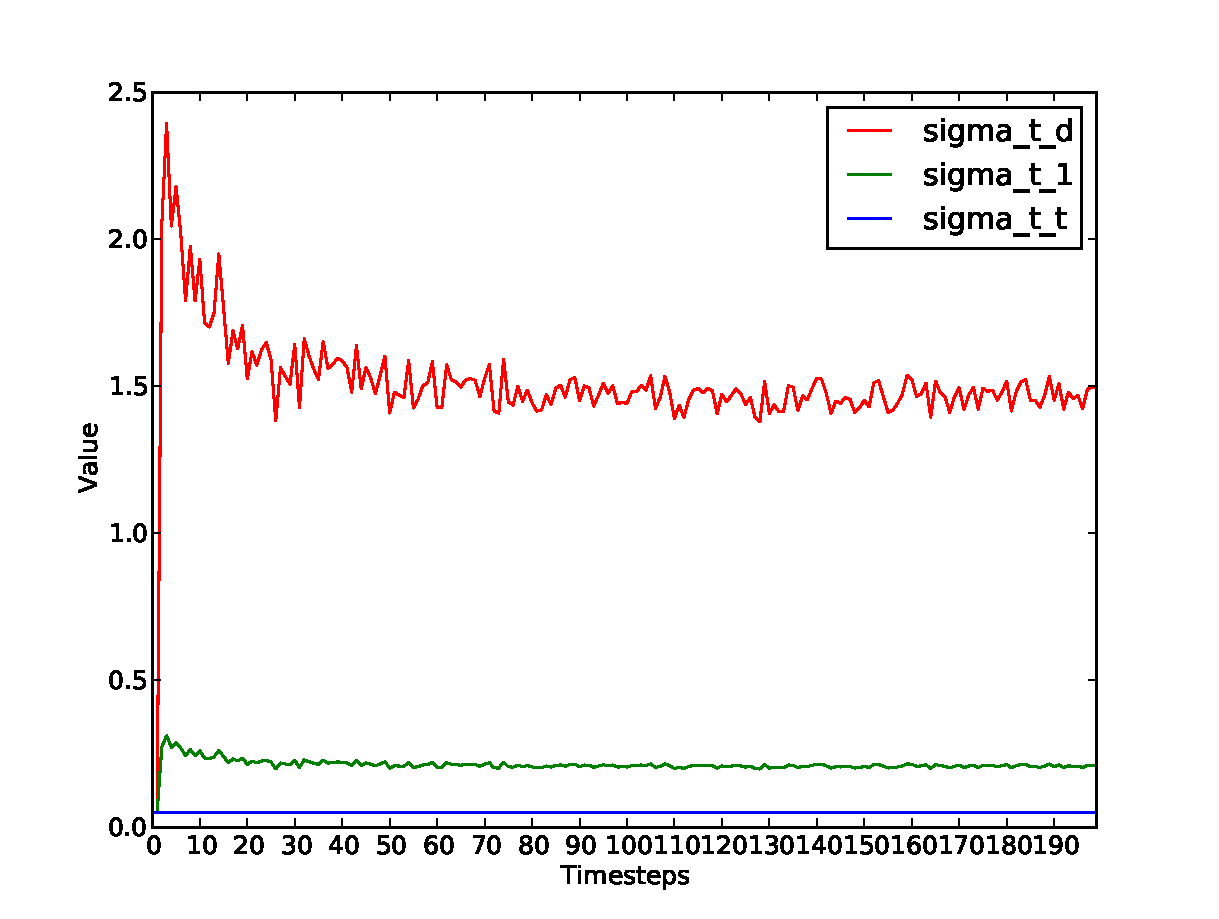
\includegraphics[height = 3.0 in]{./plots/200_005_10_s_10_motion_model_rotation.pdf}}
  \caption{\label{fig-varying_sensor_noise_motion_model_1.0_rotation}Estimate of parameter values $\sigma_{W_{v}}^{2}$, $\sigma_{W_{w}}^{2}$, $\sigma_{W_{1}}^{2}$ at every time step. The motion model noise $\sigma_{V_{v}}^{2}$ is changed from 0.05 to 1.0 at timestep 60. The sensor noise is 1.0 }
\end{figure}

\begin{figure}
  \centering
     {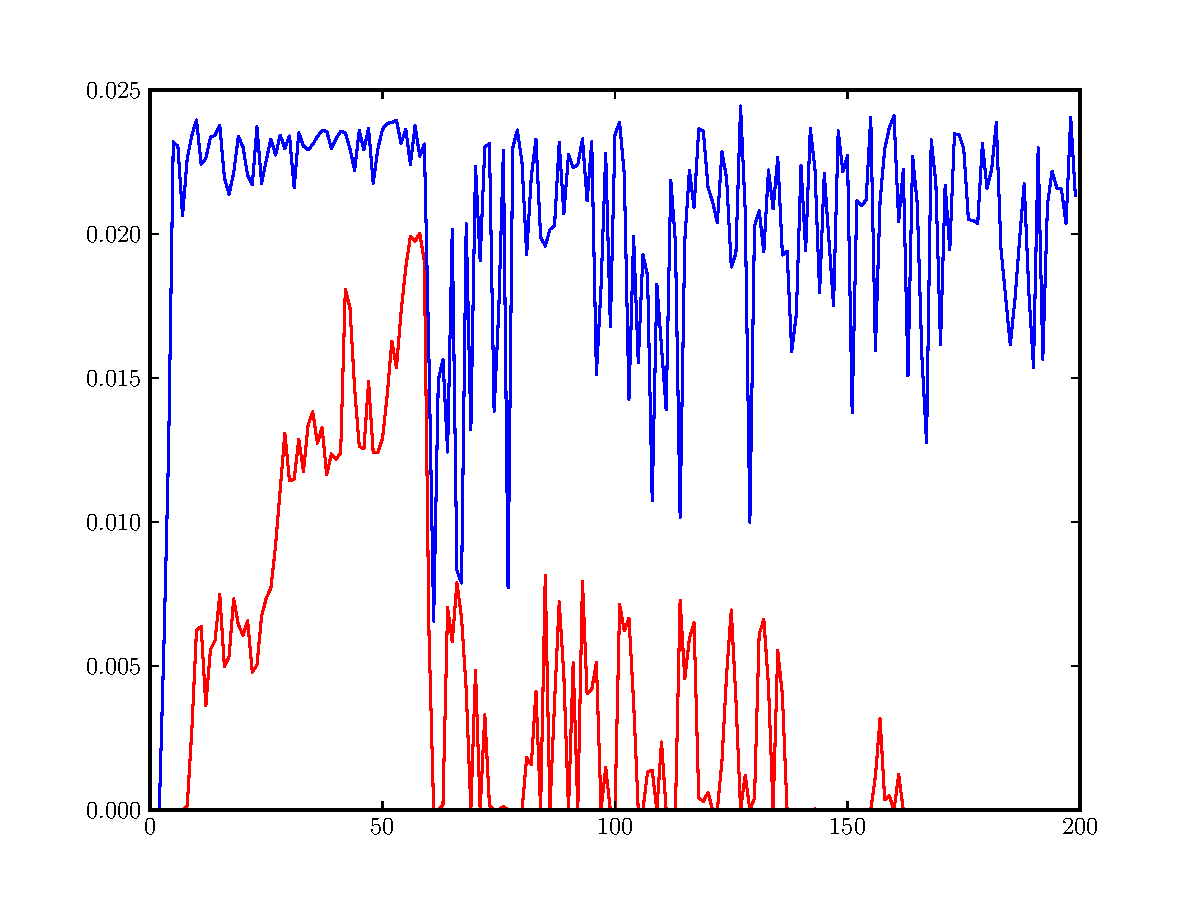
\includegraphics[height = 3.0 in]{./plots/200_005_10_s_10_max_weight.pdf}}
  \caption{\label{fig-varying_sensor_noise_sensor_model_1.0_max_weight} Difference between the maximum weight and average weight of the particles. The motion model noise $\sigma_{V_{v}}^{2}$ is changed from 0.05 to 1.0 at timestep 60. The sensor noise is 1.0}
\end{figure}

To simulate changes in the environment for the first two experiments we change $\sigma_{V_{v}}^2$. In the next two experiments we would induce drift in the system and compare both motion models in terms of localization error.

In order to simulate drift we describe the translational and rotational movement as
\begin{equation}
\label{eq- drift subtract}
V_{t}\sim\mathcal{{N}}(v_{t}-a,v_{t}^{2}\sigma_{V_{v}}^{2}+w_{t}^{2}\sigma_{V_{w}}^{2}+\sigma_{V_{1}}^{2})
\end{equation}

\begin{equation}
W_{t}\sim\mathcal{{N}}(w_{t}-b,v_{t}^{2}\sigma_{w_{v}}^{2}+w_{t}^{2}\sigma_{V_{w}}^{2}+\sigma_{W_{1}}^{2})
\end{equation}


where a and b are constants representing drifts in the system. 

\begin{figure}
  \centering
     {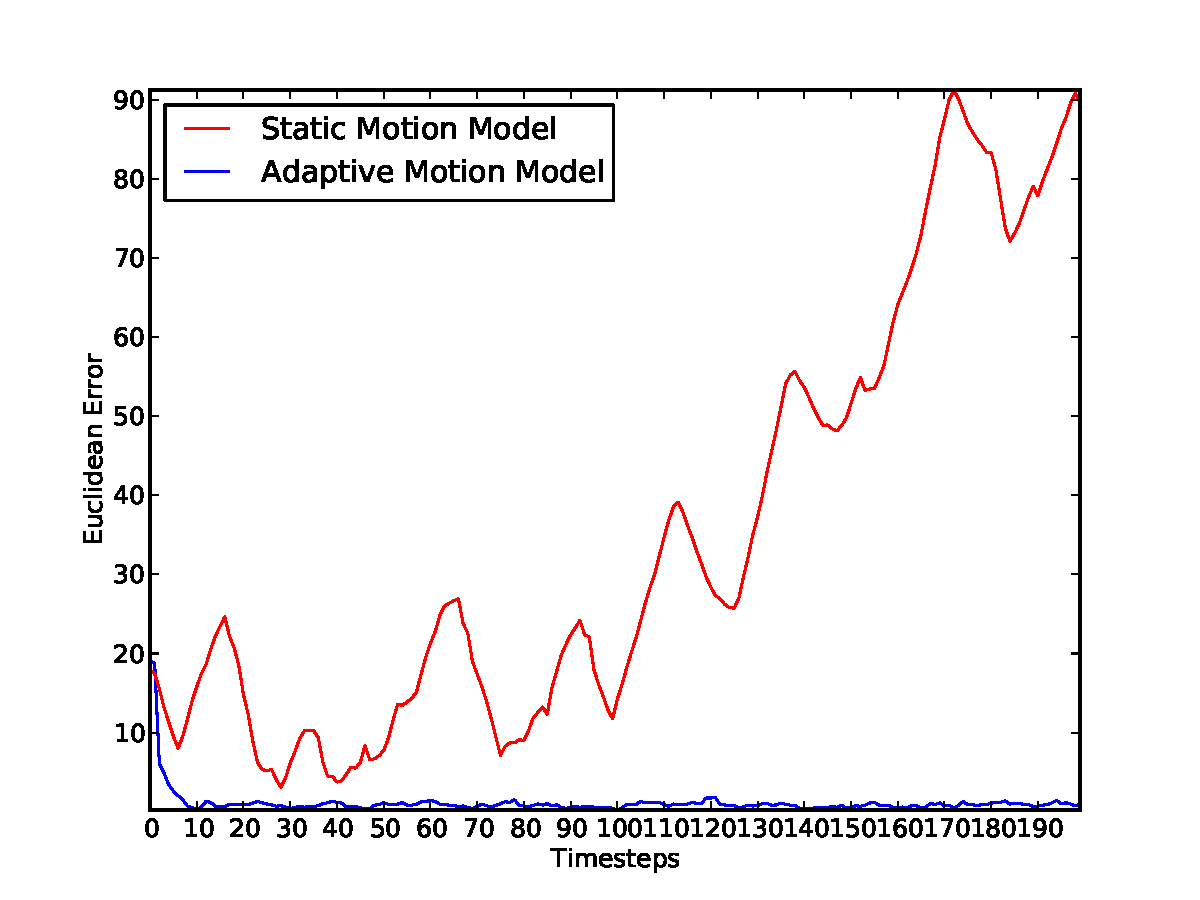
\includegraphics[height = 3.0 in]{./plots/200_005_005_s_10_traj_3_drift_20.pdf}}
  \caption{\label{fig-drift_2.0} Plot showing the localization error between robot and the estimate of the robot's location by particle filters. The drift is present throughout the experiment described by equation ~\ref{eq- drift subtract} with a=2 . The rest of the parameters remain same and the sensor noise is 1.0.}
\end{figure}
   
   
\begin{figure}
  \centering
     {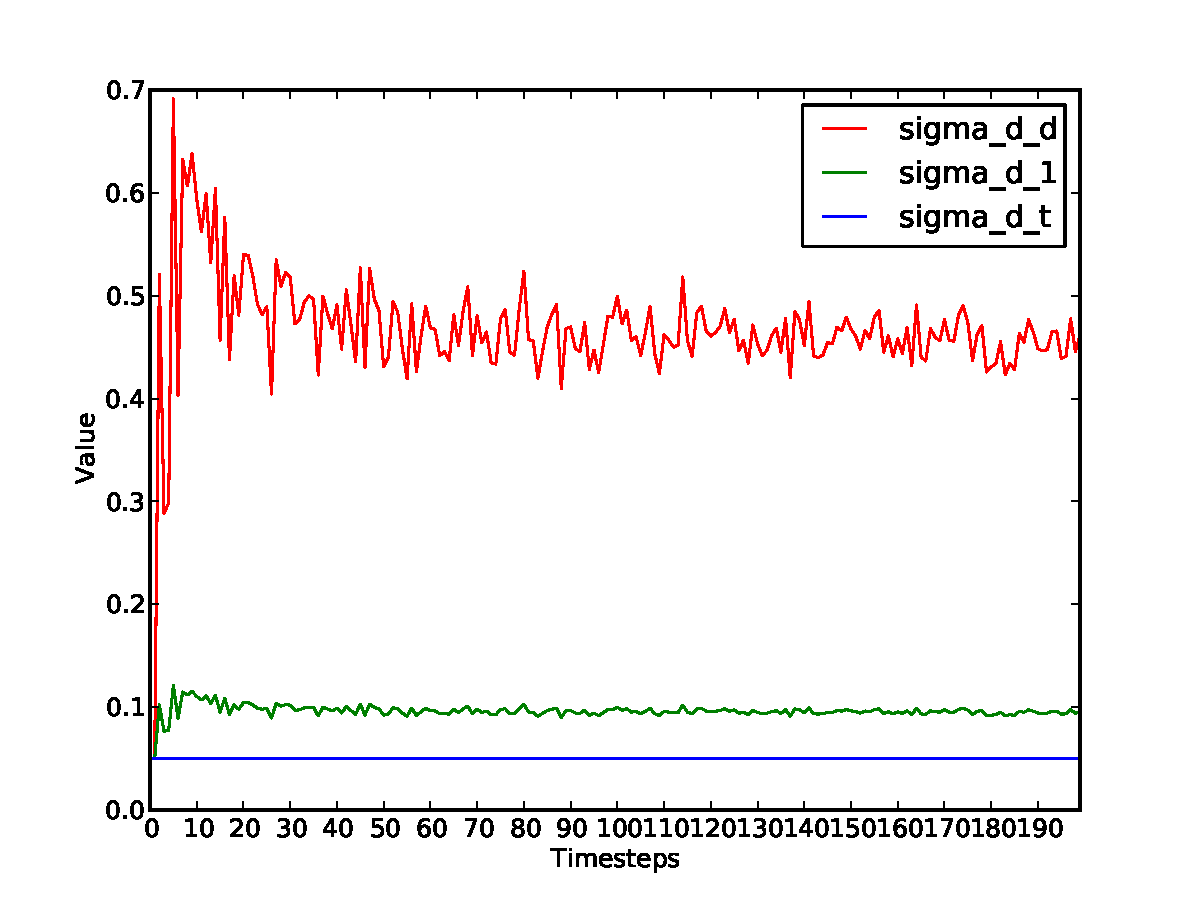
\includegraphics[height = 3.0 in]{./plots/200_005_005_s_10_traj_3_drift_20_motion_model_trans.pdf}}
  \caption{\label{fig-drift_motion_model_1.0_trans} Estimate of parameter values $\sigma_{V_{v}}^{2}$, $\sigma_{V_{w}}^{2}$,  $\sigma_{V_{1}}^{2}$ at every time step. The drift is present throughout the experiment described by equation ~\ref{eq- drift subtract} with a=2 . The rest of the parameters remain same and the sensor noise is 1.0.}
\end{figure}

\begin{figure}
  \centering
     {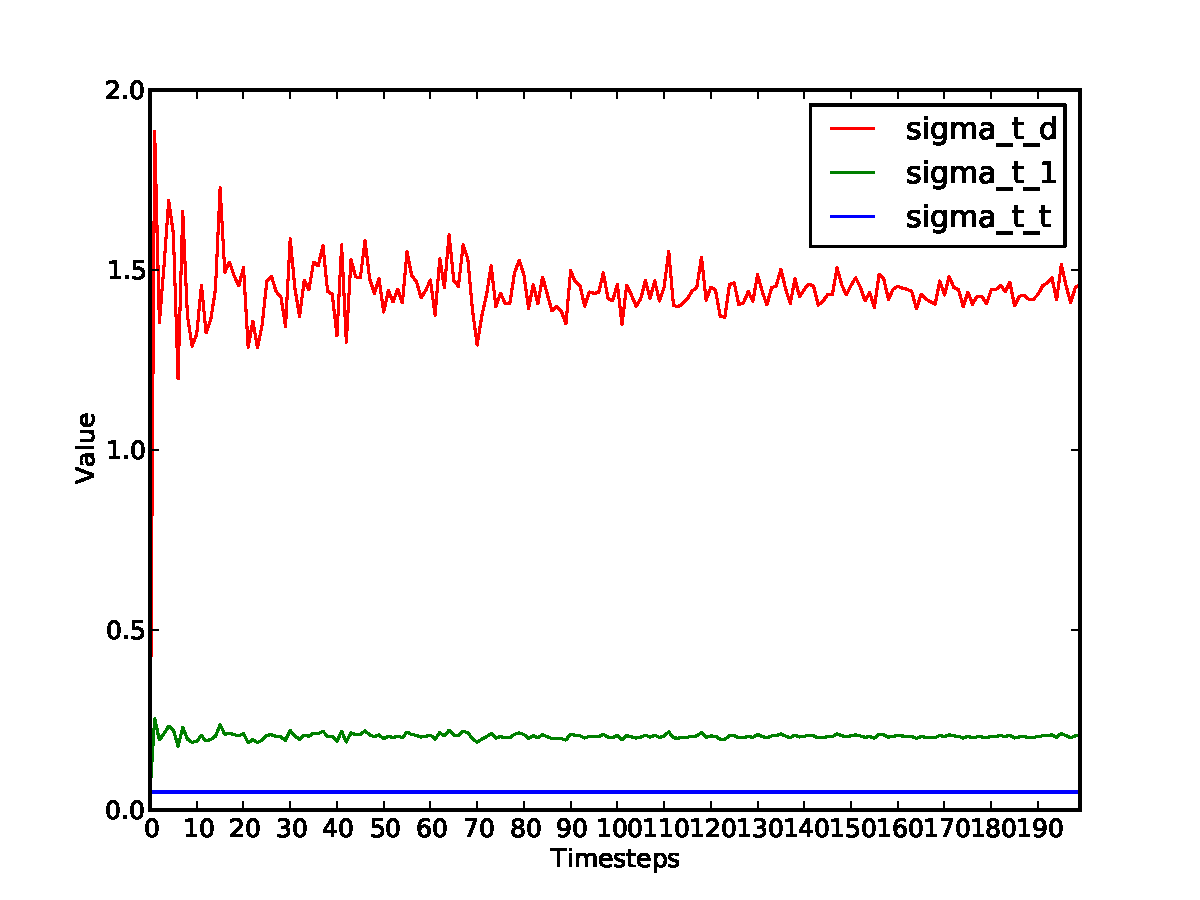
\includegraphics[height = 3.0 in]{./plots/200_005_005_s_10_traj_3_drift_20_motion_model_rotation.pdf}}
  \caption{\label{fig-drift_motion_model_1.0_rotation} Estimate of parameter values $\sigma_{V_{v}}^{2}$, $\sigma_{V_{w}}^{2}$,  $\sigma_{V_{1}}^{2}$ at every time step. The drift is present throughout the experiment described by equation ~\ref{eq- drift subtract} with a=2 . The rest of the parameters remain same and the sensor noise is 1.0.}
\end{figure}

Table ~\ref{tab-:drift} gives us a summary of the experiments performed to demonstrate the effectiveness of the algorithm to account for drift. To account for the drift we don't include an extra parameter in motion model as the variances $\sigma_{V_{v}^{2}}$, $\sigma_{V_{v}^{1}}$  should account for drift and we see that in Table ~\ref{tab-:drift}. The rest of the parameters remain unchanged. The drift is present throughout the experiment and performance of the algorithm is shown in Figure ~\ref{fig-drift_2.0}.

\begin{table}[tbh]

\centering
\begin{tabular}{|c|c|>{\centering}p{2cm}|c|c|>{\centering}p{2cm}|>{\centering}p{2cm}|}
\hline 
\multicolumn{2}{|>{\centering}p{2cm}|}{Initial Parameter Values} & Changed Parameter Values & \multicolumn{1}{>{\centering}p{2cm}|}{Estimated Parameter Values} & \multicolumn{1}{>{\centering}p{2cm}|}{Drift } & Trajectories & Sensor noise\tabularnewline
\hline 
 &  &  &  &  &  & \tabularnewline
\hline
$\sigma_{V_{v}}^{2}$ & 0.05 & 0.05 & 0.461 & 2.0 & 3 & 1.0\tabularnewline
\hline 
$\sigma_{V_{w}}^{2}$ & 0.05 & 0.05 & 0.05 &  2.0 & 3 & 1.0\tabularnewline
\hline 
$\sigma_{V_{1}}^{2}$ & 0.05 & 0.05 & 0.095 & 2.0 & 3 & 1.0\tabularnewline
\hline 
$\sigma_{W_{v}}^{2}$ & 0.05 & 0.05 & 1.460 & 2.0 & 3 & 1.0\tabularnewline
\hline 
$\sigma_{W_{w}}^{2}$ & 0.05 & 0.05 & 0.05 & 2.0 & 3 & 1.0\tabularnewline
\hline 
$\sigma_{W_{1}}^{2}$ & 0.05 & 0.05 & 0.206 & 2.0 & 3 & 1.0\tabularnewline
\hline 
\end{tabular}
\caption{\label{tab-:drift}Initial and estimated values of parameters with drift}
\end{table}

Another way to include drift in the system is 
\begin{equation}
\label{eq- drift multiply}
V_{t}\sim\mathcal{{N}}(v_{t}*a,v_{t}^{2}\sigma_{V_{v}}^{2}+w_{t}^{2}\sigma_{V_{w}}^{2}+\sigma_{V_{1}}^{2})
\end{equation}
\begin{equation}
W_{t}\sim\mathcal{{N}}(w_{t}*b,v_{t}^{2}\sigma_{w_{v}}^{2}+w_{t}^{2}\sigma_{V_{w}}^{2}+\sigma_{W_{1}}^{2})
\end{equation}


The results are described in Figure ~\ref{fig-drift_multiply} and in this case as well the drift is present throughout the experiment.
\begin{figure}
  \centering
     {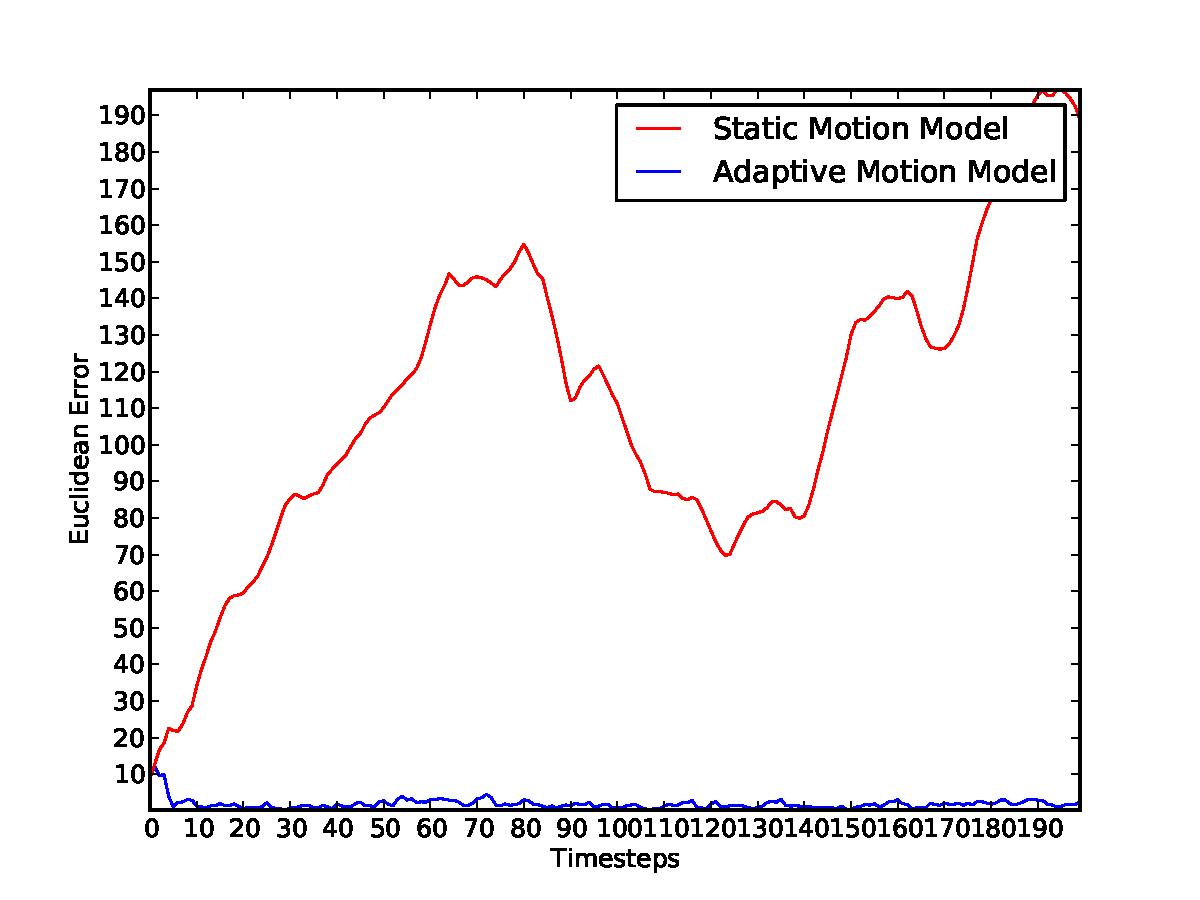
\includegraphics[height = 3.0 in]{./plots/200_005_005_s_10_traj_3_drift_20_multiply.pdf}}
  \caption{\label{fig-drift_multiply} Plot showing the localization error between robot and the estimate of the robot's location by particle filters. The drift is present throughout the experiment described by equation ~\ref{eq- drift multiply} with a=2. The rest of the parameters remain same and the sensor noise is 1.0. }
\end{figure}

In all the experiments above we assume that the sensor noise is constant through out the experiment. In practice we find that the quality of sensor readings varies with environment. For example in an AUV we won't get sonar readings throughout the mission. This could be because sometimes its difficult to find the bottom of the sea floor or sonar sensor could be switched off for some time periods to save power on the battery.

In the next experiment there are two changes at time steps 60 and 100. At time step 60 we change the motion model noise $\sigma_{V_{v}}^2$ from 0.05 to 0.5. We change the sensor noise  at time step 100 and compare the behaviour of static and adaptive motion model. After time step 100 we can see the error growing in adaptive and static motion model. The adaptive motion model quickly learns the sensor is high and starts relying on its motion model. This helps in decreasing the localization error and can be seen in Figure ~\ref{fig-different sensor noise}. In learning with a high sensor noise we are adjusting our motion model to compensate for the noise in the sensor model therfore we see an increasing estimate of the parameters (Figure ~\ref{fig-different sensor noise motion model trans}).


\begin{figure}
  \centering
     {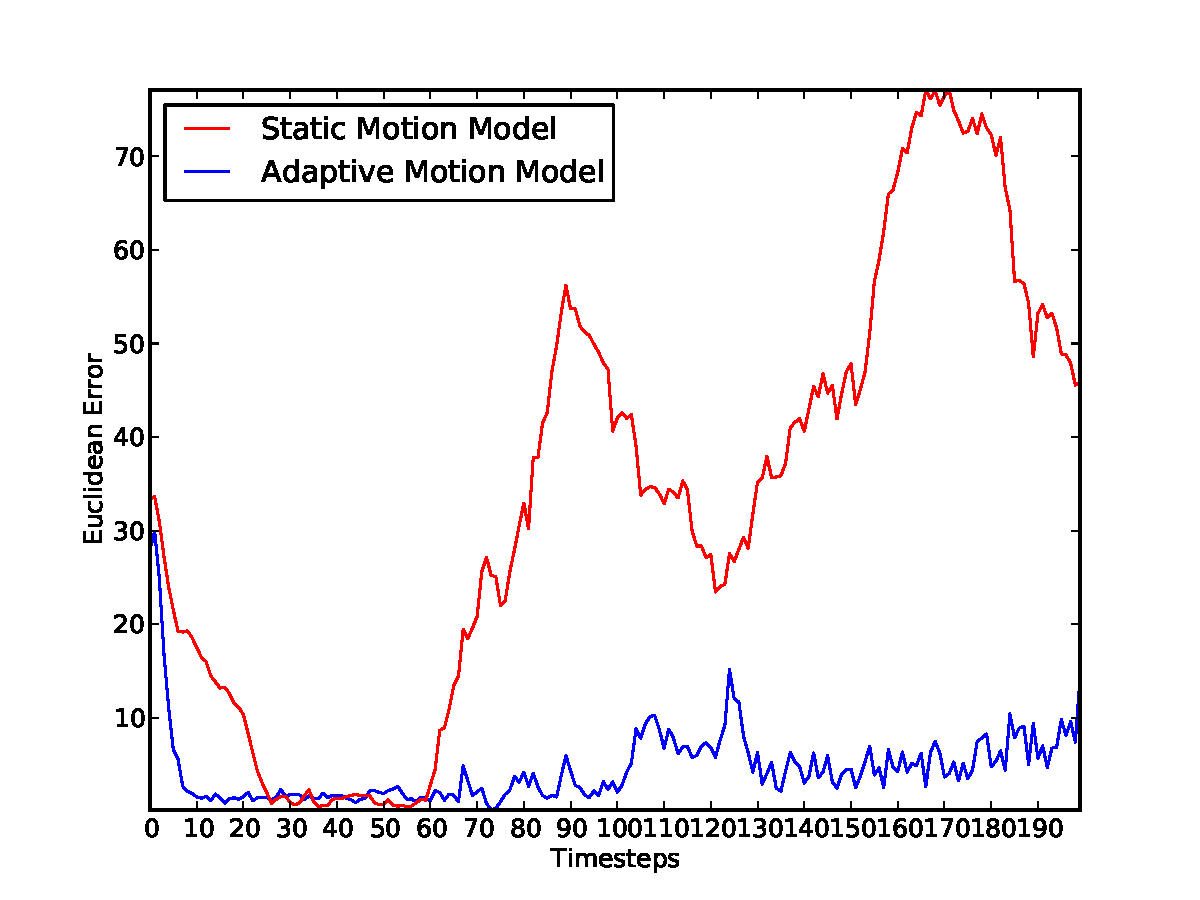
\includegraphics[height = 3.0 in]{./plots/200_005_05_s_10_100_100_traj_3_trial_1.pdf}}
  \caption{\label{fig-different sensor noise} Plot showing the localization error between robot and the estimate of the robot's location by particle filters. The $\sigma_{V_{v}}^{2}$ is changed from 0.05 to 1.0 at timestep 60. The sensor noise is changed from 1.0 to 10.0 at timestep 100. }
\end{figure}

\begin{figure}
  \centering
     {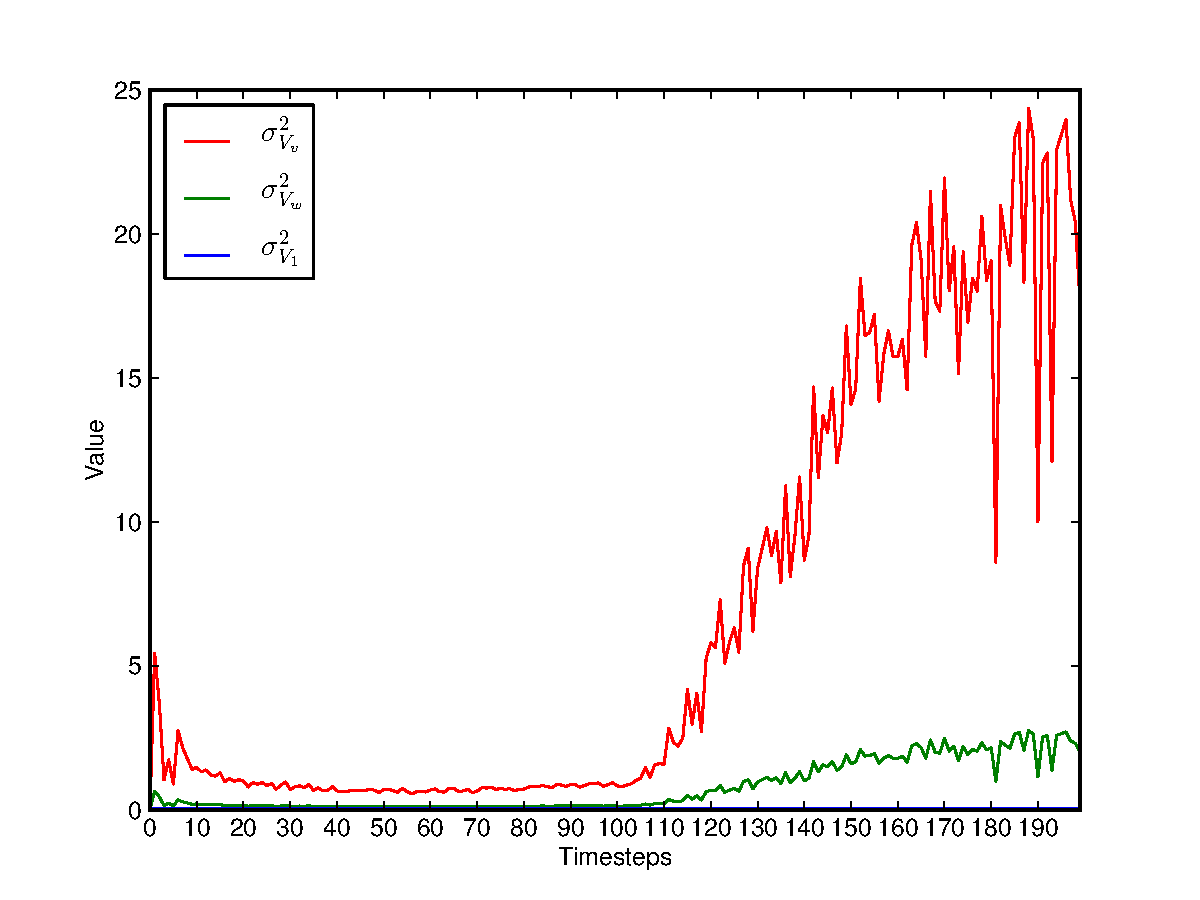
\includegraphics[height = 3.0 in]{./plots/200_005_05_s_10_100_100_traj_3_trial_1_motion_model_trans.pdf}}
  \caption{\label{fig-different sensor noise motion model trans} Estimate of parameter values $\sigma_{V_{v}}^{2}$, $\sigma_{V_{w}}^{2}$,  $\sigma_{V_{1}}^{2}$ at every time step. The $\sigma_{V_{v}}^{2}$ is changed from 0.05 to 1.0 at timestep 60. The sensor noise is changed from 1.0 to 10.0 at timestep 100.}
\end{figure}

\begin{figure}
  \centering
     {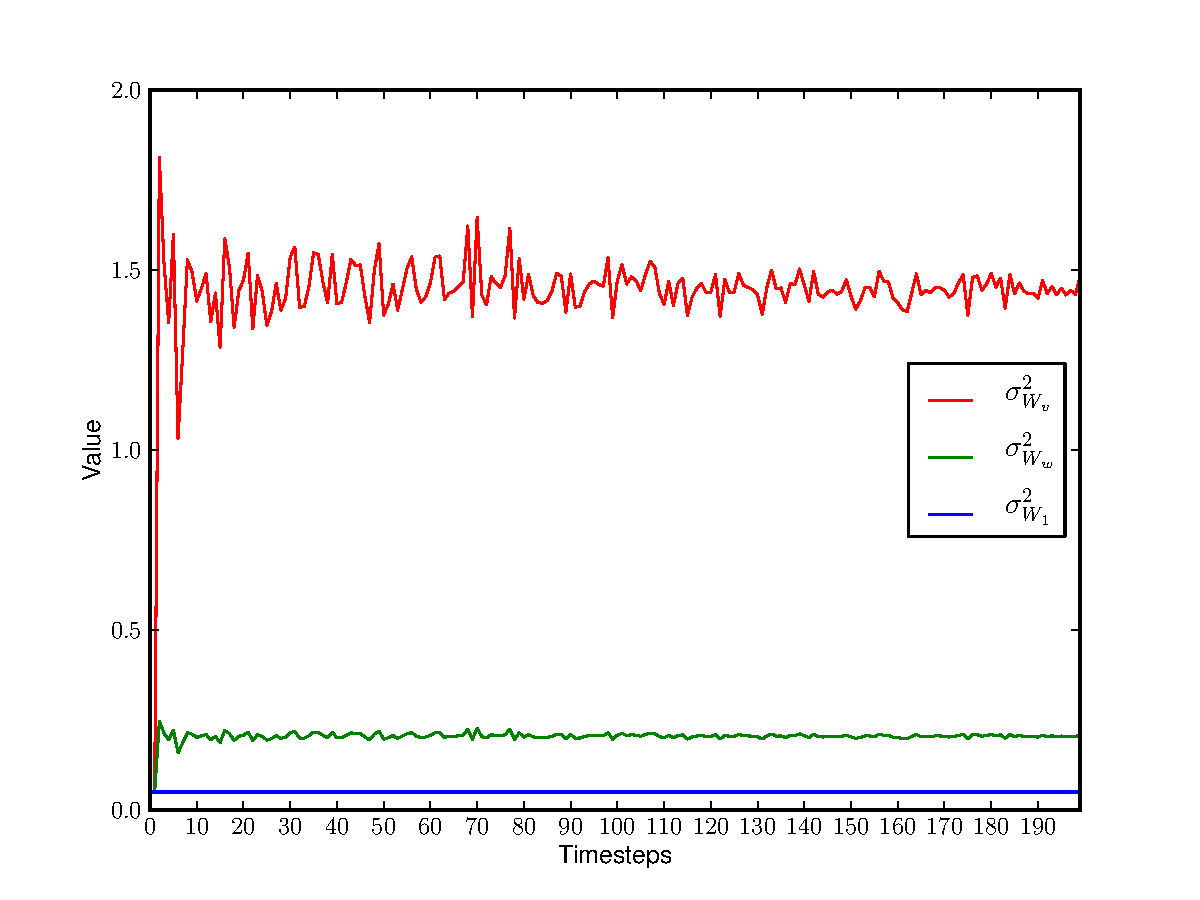
\includegraphics[height = 3.0 in]{./plots/200_005_05_s_10_100_100_traj_3_trial_1_motion_model_rotation.pdf}}
  \caption{\label{fig-different sensor noise motion model rotation}Estimate of parameter values $\sigma_{W_{v}}^{2}$, $\sigma_{W_{w}}^{2}$, $\sigma_{W_{1}}^{2}$ at every time step. The $\sigma_{V_{v}}^{2}$ is changed from 0.05 to 1.0 at timestep 60. The sensor noise is changed from 1.0 to 10.0 at timestep 100.}
\end{figure}


\chapter{Landmarks extraction using Side Sonar Images}
\section{Introduction}
The sensor model $p(z_{t}|x_{t})$ is the probability of a measurement z given the robot is at position x. Thrun \cite{thrun2005probabilistic} divides the sensors for mobile robots in five classes such as contact sensors, internal sensors, proximity sensors, visual sensors and satellite-based sensors. Examples for various classes are shown in Table ~\ref{tab-: classes of sensors}.

\begin {table}[tbh]
\begin{tabular}{|c|c|}
\hline 
Classes of Sensors & Examples of each class \\ 
\hline 
Contact Sensors & Bumpers \\ 
\hline 
Internal Sensors & Accelerometers, Gyroscopes, Compasses \\ 
\hline 
Proximity Sensors & Sonar, Radar, Laser range-finders, Infrared \\ 
\hline 
Visual Sensors  & Cameras \\ 
\hline 
Satellite Based Sensors & GPS \\ 
\hline 
\end{tabular}
\caption{\label{tab-: classes of sensors} Sensors for Mobile robots. Table taken from \cite{thrun2005probabilistic}}
\end{table}
The measurements from these sensors in a particle filter algorithm are used to assign weights aka importance factor to particles. Most common way of sensing the environment is through landmarks. The landmarks can be active beacons such as GPS or passive such as visual, retro-reflective etc. The sensors measure the distance , bearing or both from the landmarks to estimate their position in the environment. 

In our simulated experiment the sensor model assumes to have four static landmarks and at all times we can measure the distance from them. For our algorithm to work on AUV we need some sort of reference points to measure the actual movement of the vehicle. These reference points need to be computed on the fly as we don't have the liberty of having static maps for underwater environments. As my algorithm deals with cases in which AUV doesn't loop back and we have limited field of view we need dynamic landmarks for our sensor model. To extract dynamic landmarks we used side sonar images and run feature extraction techniques such as SIFT on the images. These extracted landmarks can be used as reference points for our algorithm to adapt motion model for AUV.

The dynamic landmarks algorithm for side sonar images is not integrated in the simulated experiment described in Chapter ~\ref{ch-: results adapting motion model}. This is because of the unavailability of the motion data such as recording of IMU, DVL etc for AUV. To validate our algorithm for dynamic landmarks we extract motion information from real side sonar data and compare it to the total distance moved by the AUV. In the next two section I describe how side scan sonar and SIFT works. In section ~\ref{ch-: dynamic landmarks} the algorithm to compute landmarks is presented and Chapter ~\ref{ch-: results motion estimation} contains the results of the algorithm.  



\subsection{Side Scan Sonar} 
Side scan sonar is used to create pictures or an image of the sea floor. A side scan sonar sensor is shown in Figure ~\ref{fig- side scan sonar sensor}. It measures of how "loud" the return echo is and paints a picture (1). In the sea floor we find  hard areas such as rock and soft areas such as sand. The hard areas are represented by darker areas in the image as they return a stronger signal as compared to a soft area. A typical side sonar image is shown in Figure ~\ref{fig- side scan sonar image}. Side scan sonar is the only imaging tool that works at low depth therefore we use it to extract landmarks for adapting the motion model. Sound waves travel very effectively in water as compared to light therefore at lower depths sonar is used to image the sea floor instead of cameras. 
\begin{figure}
  \centering
     {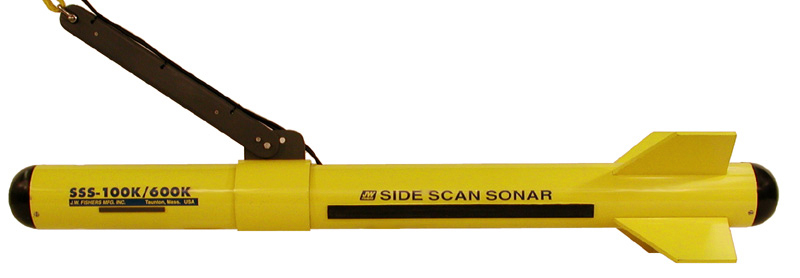
\includegraphics[height = 3.0 in]{/home/rohan/Documents/thesis/thesis_writeup/side_scan_sonar_sensor.jpg}}
  \caption{\label{fig- side scan sonar sensor} Side scan sonar sensor using dual frequency made by JW Fishers . Image taken from \cite{side_sonar_fisheries_url}}
\end{figure}

\begin{figure}
  \centering
     {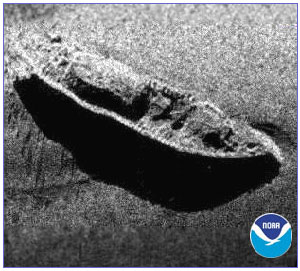
\includegraphics[height = 3.0 in]{/home/rohan/Documents/thesis/thesis_writeup/side_scan_sonar.jpg}}
  \caption{\label{fig- side scan sonar image} Side scan sonar image of the wreck. Image taken from \cite{side_sonar_url}}
\end{figure}

Side-scan transmits sound energy and analyzes the echo that is bounced off from the sea floor or other objects. It typically consists of three basic components: towfish, transmission cable and topside porcessing unit. It emits pulses in the shape of cone or fan to either sides of the towfish, typically to a distance of 100 meters. The angular dimensions of these beams are designed to be narrow along-tack and wide across track to cover as much seabed range as possible.  The echoed sound waves are received by transducers and are continuously recorded. Each pulse shows a narrow stip below and to the sides.  The recorded echos are put together along the direction of motion to form images of the seafloor. The sound frequencies range from 100 to 500 Khz in side scan sonar; higher frequencies yield better resolution but less range. Currently in the market there are systems with dual frequency which allow the opeator to use high frequency to produce sharper images or lower frequencies to cover greater depths. Side scan 
systems can be characterized according to their operating frequency \cite{side_sonar_usgs_url}.

\begin{table}

\begin{tabular}{|c|c|c|c|}
\hline 
Sidescan Sonar Type & Frequency & Wavelenght & Range \\ 
\hline 
"Low" & 5 kHz & 30 cm & >50 km \\ 
\hline 
"Low" & 10 kHz & 15 cm & 10 km \\ 
\hline 
"Low" & 25 kHz & 6 cm & 3 km \\ 
\hline 
"Medium" & 50 kHz & 3 cm & 1 km \\ 
\hline 
"Medium" & 100 kHz & 1.5 cm & 600 m \\ 
\hline 
"Medium" & 200 kHz & 0.75 cm & 300 m \\ 
\hline 
"High" & 500 kHz & 3 mm & 150 m \\ 
\hline 
"High" & 1 mHz & 1.5 mm & 50 m \\ 
\hline 
\end{tabular} 
\caption{\label{tab-: classification of side scan} Characterization of Sidescan system according to their operating frequency. Table taken form \cite{side_sonar_usgs_url}} 
\end{table}
It can be used fisheries research, environmental studies and military applications such as mine detection. 

\begin{figure}
  \centering
     {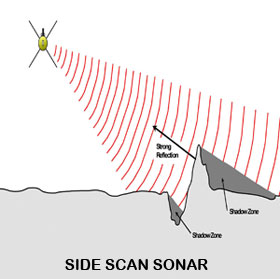
\includegraphics[height = 3.0 in]{/home/rohan/Documents/thesis/thesis_writeup/work_side_scan.jpg}}
  \caption{\label{fig- side scan sonar working} Working of a side scan sonar. Image taken from \cite{side_sonar_url}}
\end{figure}

\subsection{Scale Invariant Feature Transform}
SIFT is an algorithm in computer vision to detect and describe local feature of an image that are not affected by scaling and rotation. It was first proposed by David Lowe in 1999 \cite{lowe1999object} and has been used for object recognition, robotic mapping and navigation, image stitching, video tracking etc.

The first step in SIFT is to construct scale space i.e. create internal representations of the original image to ensure scale in variance. In SIFT progressively blurred out images are generated using the original image. In the next step you the original image is resized to half of its size and again the blurred out images are generated. 

\begin{figure}
  \centering
     {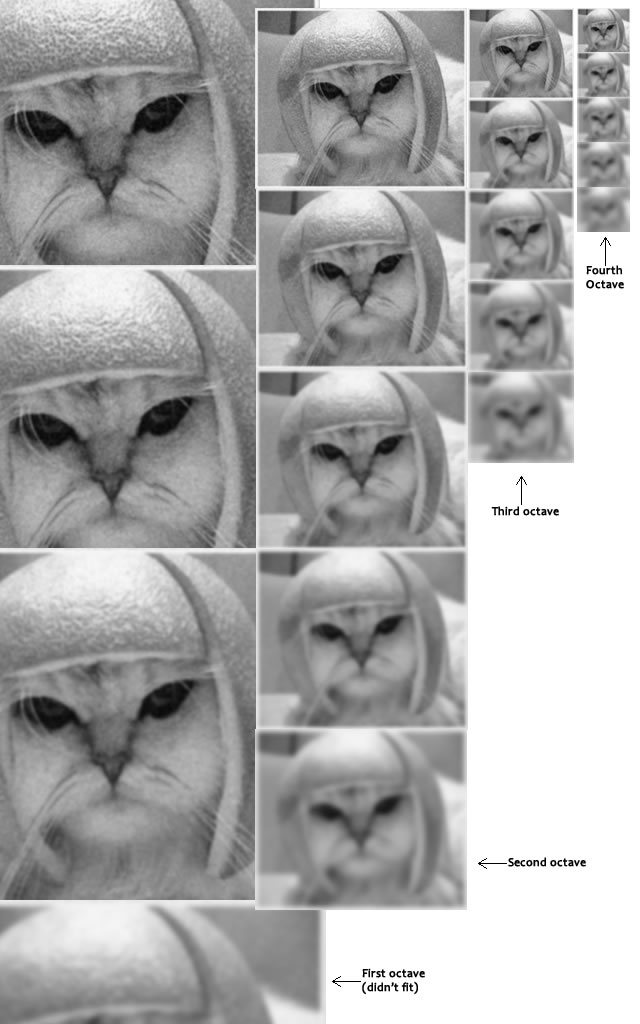
\includegraphics[height = 3.0 in]{/home/rohan/Documents/thesis/thesis_writeup/sift-octaves.jpg}}
  \caption{\label{fig- sift octaves} Representation of what Octaves look like in SIFT. Image taken from \cite{sift_url}}
\end{figure}

The images of same size are grouped together and belong to an octave. In figure ~\ref{fig- sift octaves} there are four octave and each octave has five images. The number of octaves depends upon the original size of the image. The blurring of images in each octave can be represented mathematically by 

\begin{equation}
L(x,y,\sigma) = G(x,y,\sigma) * I(x,y)
\end{equation}
where L is the blurred image , G is the Gaussian blur operator, I is an image, x,y are the location coordinates and $\sigma$ is the scale parameter. The $*$ is the convulation of Gaussian blur G onto the image I. 
The next step is to find another set of images by Difference of Gaussian (DOG) which help us in finding out the interesting keypoints in the image. In this step we calculate the difference between two consecutive scales as shown in Figure ~\ref{fig- sift dog}. This process is done at every octave. 

\begin{figure}
  \centering
     {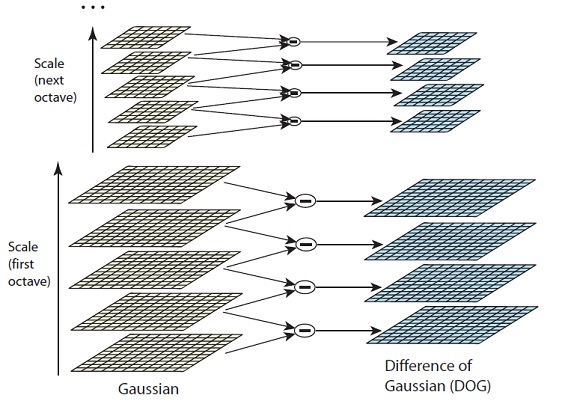
\includegraphics[height = 3.0 in]{/home/rohan/Documents/thesis/thesis_writeup/sift-dog-idea.jpg}}
  \caption{\label{fig- sift dog} Difference of Gaussian done to caluclate keypoints in the image. Image taken from \cite{sift_url}}
\end{figure}

To put this concept in our example the DOG is applied to cat images and the output is shown in Figure ~\ref{fig- sift dog images}. 
\begin{figure}
  \centering
     {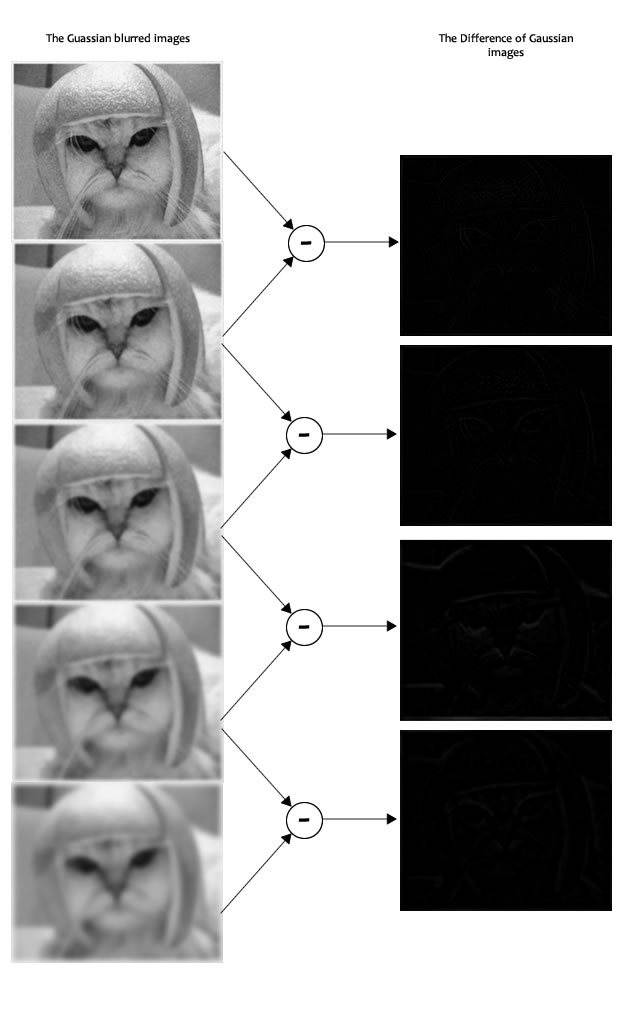
\includegraphics[height = 3.0 in]{/home/rohan/Documents/thesis/thesis_writeup/sift-dog-images.jpg}}
  \caption{\label{fig- sift dog images} Applying DOG on a set of images present in a single octave. Image taken from \cite{sift_url}}
\end{figure}

After calculating the DOG images we can find the keypoints in two steps. Firstly locate the maxima/minima in DOG images. Secondly find subpixel maxima/minima. In the first step the algorithm iterates through each pixel and all the neighbors are checked. This process is explained in Figure 

\begin{figure}
  \centering
     {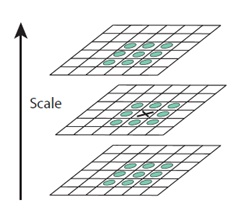
\includegraphics[height = 3.0 in]{/home/rohan/Documents/thesis/thesis_writeup/sift-maxima-idea.jpg}}
  \caption{\label{fig- maxima and minima sift octaves} Locate maxima/minima in DOG images. X marks the current pixel and it is compared with its 26 neighbors. Image taken from \cite{sift_url}}
\end{figure}

In the figure X is the current pixel and the green circles represent the neighbors. X is marked as a keypoint if it is the greatest or least of all neighbors. These are approximate as mostly the maxima/minima never lies on a pixel. To access the data "between" pixels we need to calculate the subpixel location. This can be done by Taylor expansion of the image around the approximate keypoint. It can be mathematically represented by 

\begin{equation}
D(x) = D + \tfrac{\partial D^{T}}{\partial x}x+\tfrac{1}{2}x^{T}\tfrac{\partial^{2} D}{\partial x^{2}}x
\end{equation}

After generating a set keypoints we need to get rid of points whihc have low contrast features and are present on an edge. The algorithm checks for intensity value at the pixel location of the keypoint and if it is less than a certain value if is rejected. To remove edges the perpendicular gradients are calculated at the keypoint. If both the gradients are small it is a flat region. If one gradient is big and other is small it is a edge. If both the gradients are big then it is a corner. The keypoints with both big gradients are considered to be a keypoint otherwise they are rejected. The SIFT algorithm can check a point is a corner or not by using a Hessian matrix. After completing this step we have a set of legitimate keypoints which are scale invariant. The next step is assign orientation to each keypoint so that they are rotation invariance. 

In this step SIFT calculates gradient magnitudes and directions around each keypoint. To perform this a histogram is created with 36 bins (each 10 degrees) representing 360 degrees of orientation. Suppose the gradient direction at a certain point is 20.56 degrees then it will go in 20-29 degree bin. The amount that is added to the bin is proportional to the magnitude of the gradient of the point. This process is repeated for all the pixels around the keypoint and in the end histogram would peak at some point. In Figure ~\ref{fig- sift bin histogram} it peaks at 20-29 degrees therefore the keypoint is assigned to third bin. In the Figure we also see that there is another peak which is above $80 \%$ of the highest peak. In this case the peak converted into a new keypoint. This new keypoint has the same location and scale as the original but has a different orientation. 

\begin{figure}
  \centering
     {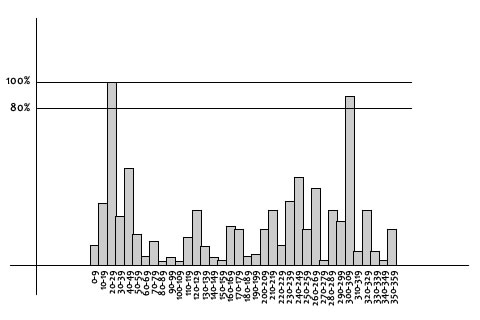
\includegraphics[height = 3.0 in]{/home/rohan/Documents/thesis/thesis_writeup/sift-orientation-histogram.jpg}}
  \caption{\label{fig- sift bin histogram} Histogram describing the bins for assigning orientation to the keypoint. Image taken from \cite{sift_url}}
\end{figure}

In the final step of SIFT algorithm a unique fingerprint for a keypoint aka descriptor is calculated. To calculate the gradient we take $16 X 16$ window around the each keypoint. This $16 X 16$ window is broken into sixteen $4 X4$ windows (Figure ~\ref{fig- sift bin fingerprint}).

\begin{figure}
  \centering
     {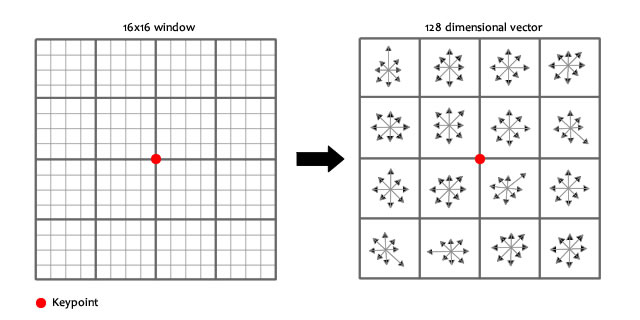
\includegraphics[height = 3.0 in]{/home/rohan/Documents/thesis/thesis_writeup/sift-fingerprint.jpg}}
  \caption{\label{fig- sift bin fingerprint} A $16 X16$ window is taken around a keypoint. This window is broken into sixteen $4 X 4$ windows. Image taken from \cite{sift_url}}
\end{figure}

In each window gradient magnitudes and orientations are calculated and are put in a 8 bin histogram (Figure ~\ref{fig- sift bin histogram gradient}). For examples a gradient orientation in the range of 0-44 degrees is put in the first bin. The amount added to the bin depends upon the magnitude of the gradient and the distance from the keypoint. The gradients that are far away from the keypoint will add smaller values to the bin. This can be performed using "Gaussian weighting function". 

\begin{figure}
  \centering
     {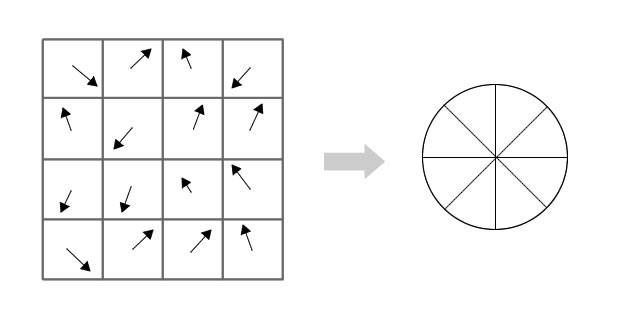
\includegraphics[height = 3.0 in]{/home/rohan/Documents/thesis/thesis_writeup/sift-4x4.jpg}}
  \caption{\label{fig- sift bin histogram gradient} The gradient orientation is assinged to 8 bin histogram. The value depends upon the magnitude of the orientation and distance from the keypoint. Image taken from \cite{sift_url}}
\end{figure}

This is done for all 16 pixels therefore you end up with $4X4X8=129$ numbers. The numbers are normalized and form the feature vector. This feature vector gives a unique identity to the keypoint. To achieve rotation independence the keypoint rotation is subtracted from each orientation therefore each gradient orientation if relative to the keypoints orientation. For illumination independence we threshold any numbers that are big and the resultant feature vector is normalized again. 

After we calculate the descriptors for each keypoint we have a set of features that describes the image and these can be used for various image processing tasks such as image matching, stitching etc. 

SIFT has  been widely used in various robotic applications. Stephen Se et. al \cite{se2001vision} proposed an vision based algorithm to localize a robot and map the environment using SIFT features. Various algorithm have been proposed to estimate motion from camera images using SIFT features \cite{barfoot2005online} \cite{scaramuzza2008appearance}. Similar algorithms have been proposed to estimate motion underwater using camera images \cite{Silva}.

Andrew Vardy et. al \cite{vandrish2011side} compared various image registration techniques for side sonar images such as  maximization of mutual information, log-polar cross-correlation, SIFT and phase correlation. He presented results and concluded that SIFT and phase-correlation provide the best performance among all the techniques. Peter King \cite{king2012real} described an algorithm to generate images from side scan sonar pings in real time. To implement my algorithm on AUV we can use the algorithm proposed by them as a black box.


\section{Dynamic Landmarks}
\label{ch-: dynamic landmarks}

As stated above we need reference points to adapt our motion model. These reference points need to be dynamic as we are learning online and we don't loop back on AUV`s route. To generate landmarks on side sonar images a preprocessing step is required to get rid of horizontal lines produced spurious electrical noise in the transducers. The noisy side sonar images is shown in Figure ~\ref{fig- side sonar image original}.

\begin{figure}
  \centering
     {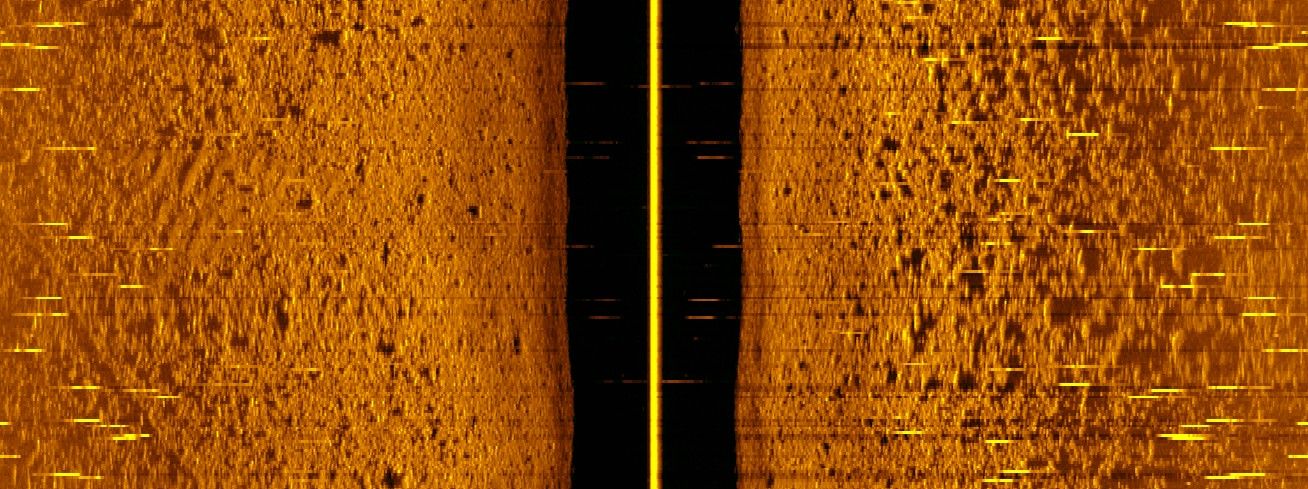
\includegraphics[height = 3.0 in]{/home/rohan/Documents/thesis/thesis_writeup/side_sonar_original.jpg}}
  \caption{\label{fig- side sonar image original} Image produced by Side scan sonar. Images produced from dataset provided by DRDC.}
\end{figure}


The preprocessing step involves using a median filter on the image to get rid of the noise. The preprocessed image is shown in Figure ~\ref{fig- side sonar median}.
\begin{figure}
  \centering
     {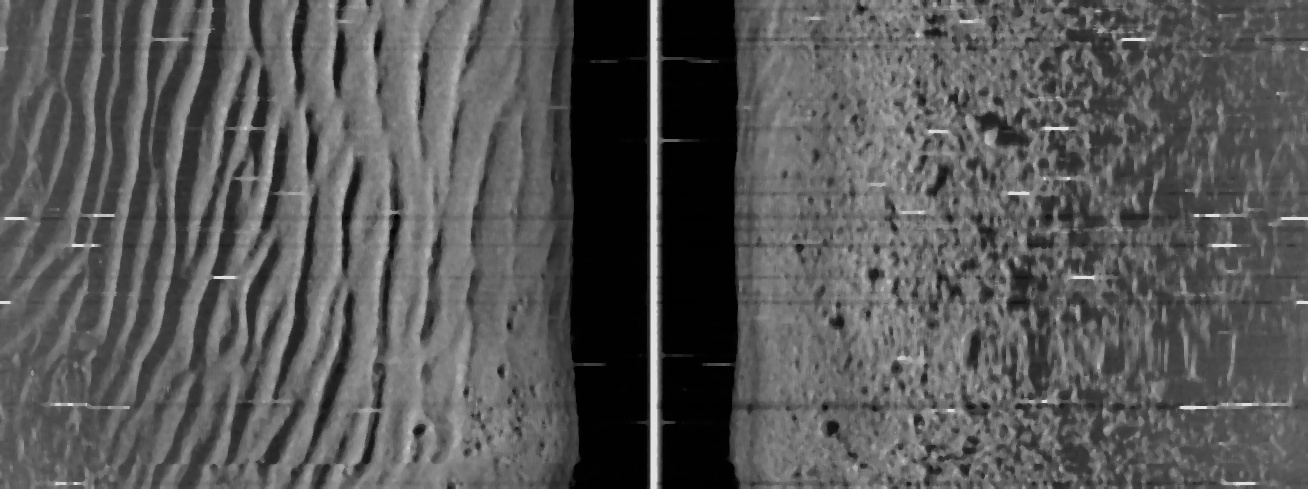
\includegraphics[height = 3.0 in]{/home/rohan/Documents/thesis/thesis_writeup/median_filter_sonar.jpg}}
  \caption{\label{fig- side sonar median} Median filter applied to side sonar image.}
\end{figure}

The disadvantage of this step is we loose information because the image is blurred. The blurred image won't give us meaningful keypoints therefore in the preprocessed image we see some horizontal lines due to restricted use of the filter. In order to get rid of all the lines we can increase the size of filter but the image will be very blurred as shown in Figure ~\ref{fig- side sonar median high}.
\begin{figure}
  \centering
     {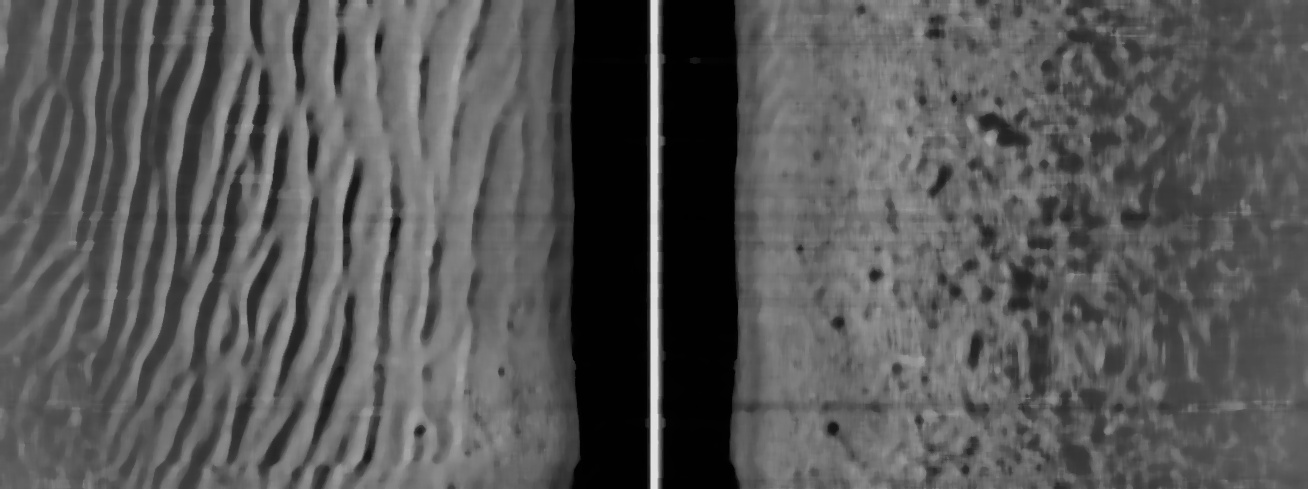
\includegraphics[height = 3.0 in]{/home/rohan/Documents/thesis/thesis_writeup/median_filter_sonar_high.jpg}}
  \caption{\label{fig- side sonar median high} Median filter with high size applied to side sonar image.}
\end{figure}

The preprocessed image is used to extract landmarks for the AUV. To generate landmarks we use feature extraction techniques such as SIFT. Figure ~\ref{fig- side sonar sift} shows the keypoints generated by SIFT using a high hessian threshold. These keypoints can be used as landmarks to adapt our motion model. We need to keep in mind that we need a high hessian threshold or else the algorithm will generate hundreds of landmarks as shown in Figure ~\ref{fig- side sonar sift high}.
\begin{figure}
  \centering
     {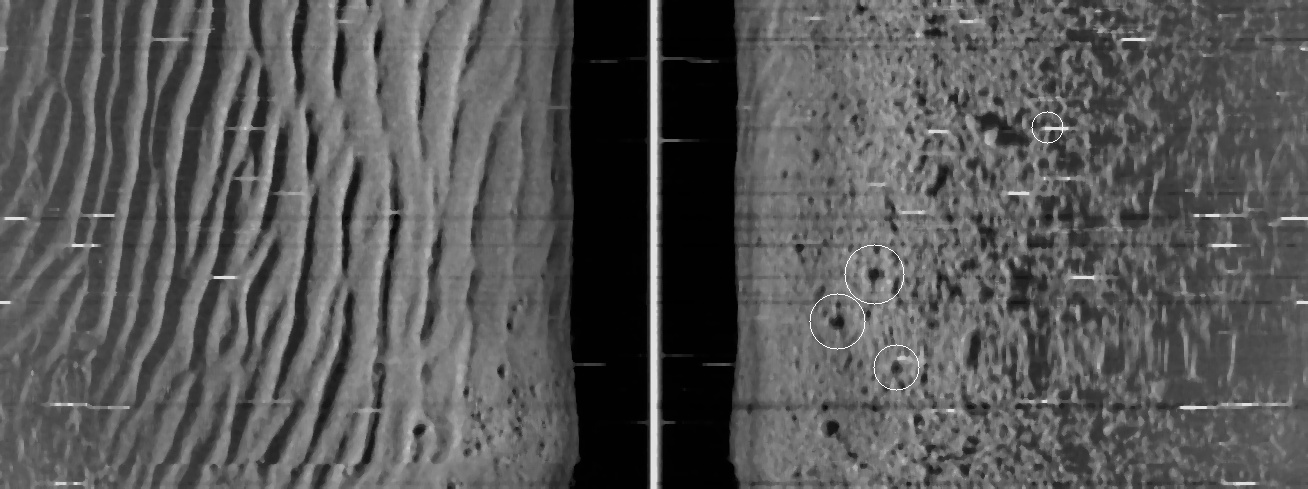
\includegraphics[height = 3.0 in]{/home/rohan/Documents/thesis/thesis_writeup/image_original_sift.jpg}}
  \caption{\label{fig- side sonar sift} SIFT features on a side sonar image.}
\end{figure}

\begin{figure}
  \centering
     {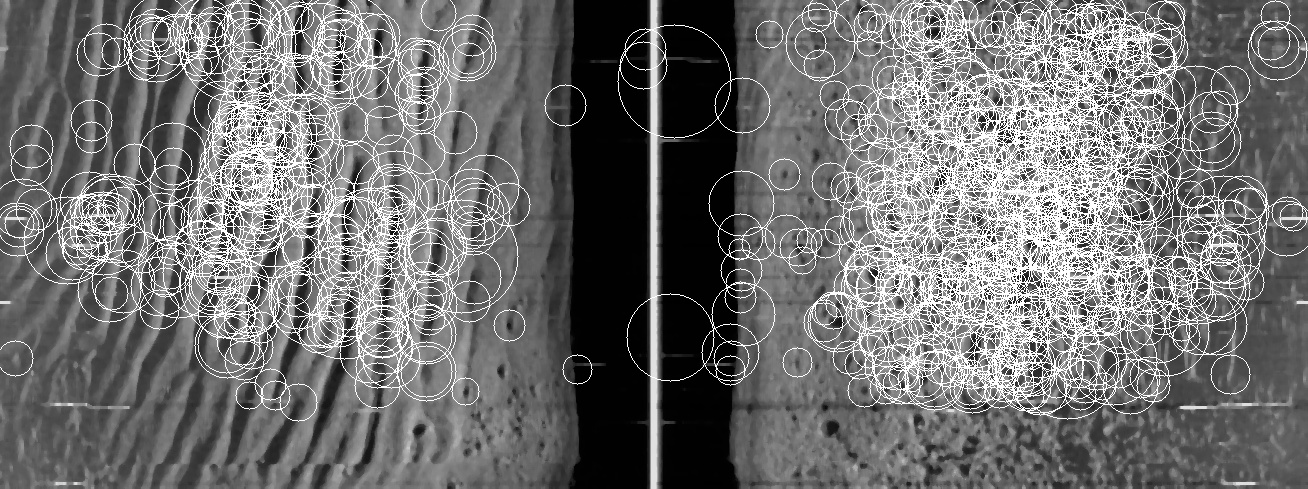
\includegraphics[height = 3.0 in]{/home/rohan/Documents/thesis/thesis_writeup/image_original_sift_high.jpg}}
  \caption{\label{fig- side sonar sift high} SIFT features on a side sonar image with low hessian threhold.}
\end{figure}


The distance of the AUV to landmarks in x-y plane can be measured. Similarly the distance of the particle filter estimate to the landmarks can be measured. Both the measured distances can be compared and used to assign weights to the particles. 

Using dynamic landmarks allows our adaptive motion model algorithm independence from a static map and helps us in learning on the fly.  

\section{Motion Estimation using side sonar images}

In mobile robots the position and orientation is determined through wheel encoders and velocity estimates. These techniques do not generalize well as they cannot be applied every robot as well as the estimates drift over time. Motion estimation using visual sensors such as camera are not restricted to particular locomotion and doesn't suffer from drift. There has been a lot of work done in estimating motion using camera images on land robots \cite{barfoot2005online} \cite{scaramuzza2008appearance}. Silvia \cite{Silva} proposed an algorithm for AUV which used camera images and SIFT to estimate motion. 

In AUV the motion estimates from INS suffer from drift and are coupled with DVL to give a better estimate of the position. Hegreneas \cite{hegrenaes2008model} combined the knowledge of vehicle dynamics to aid INS systems. In a similar manner visual motion information can be used to aid INS systems. The visual input to the dead reckoning algorithm has its pros and cons. The main advantage of using a visual estimate is that it doesn't suffer from drift which is prime concern for underwater vehicles. The disadvantage lies in the fact that we don't have side sonar images available every time. The second disadvantage is the computation power available on AUV. To specifically deal with the problems we use a high Hessian threshold to extract maximum of 4 landmarks so that feature matching is not computationally expensive.    

We verify our dynamic landmark approach by estimating motion information from side sonar images and compare it to reported movement by DVL. To generate keypoints we run SIFT on the side sonar images. We use a high hessian threshold so that we can restrict the amount of keypoints. These keypoints are matched with keypoints of the next consecutive image using a KNN based matcher. Figure ~\ref{fig- matched images} shows two consecutive images that are used to estimate motion of the AUV. In the first image the keypoints are marked in white circles. These keypoints are matched with the second image and the matched keypoints are marked in black circles. The $x$ and $y$ position of the matched keypoints is compared to the original keypoints. This gives us motion estimate of the AUV. 

\begin{figure}
  \centering
  \subfigure[a]{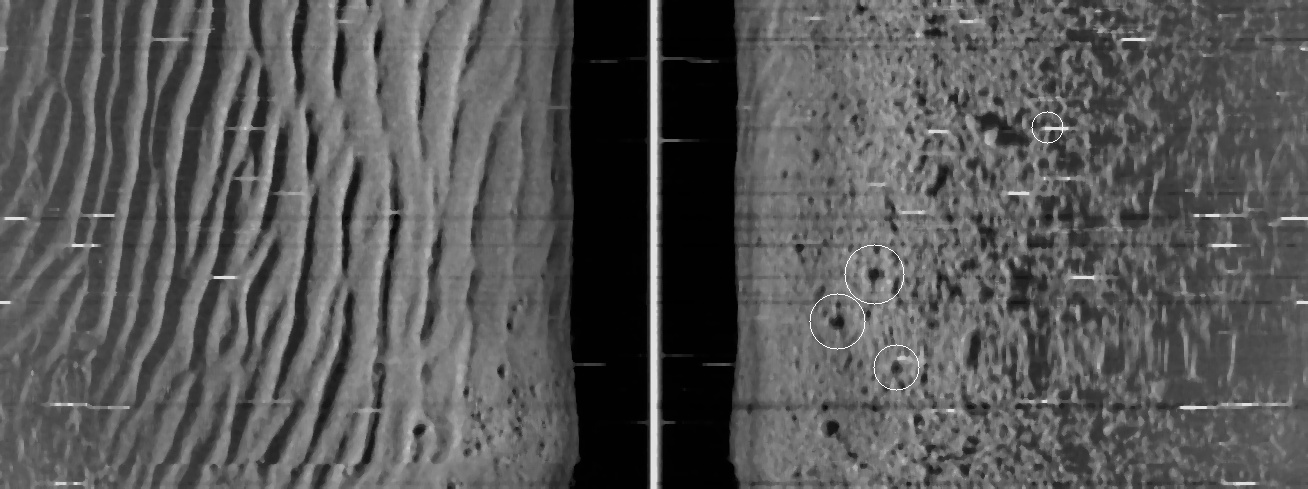
\includegraphics[width = 2.75 in]{/home/rohan/Documents/thesis/thesis_writeup/image_original_sift.jpg}}\qquad
  \subfigure[b]{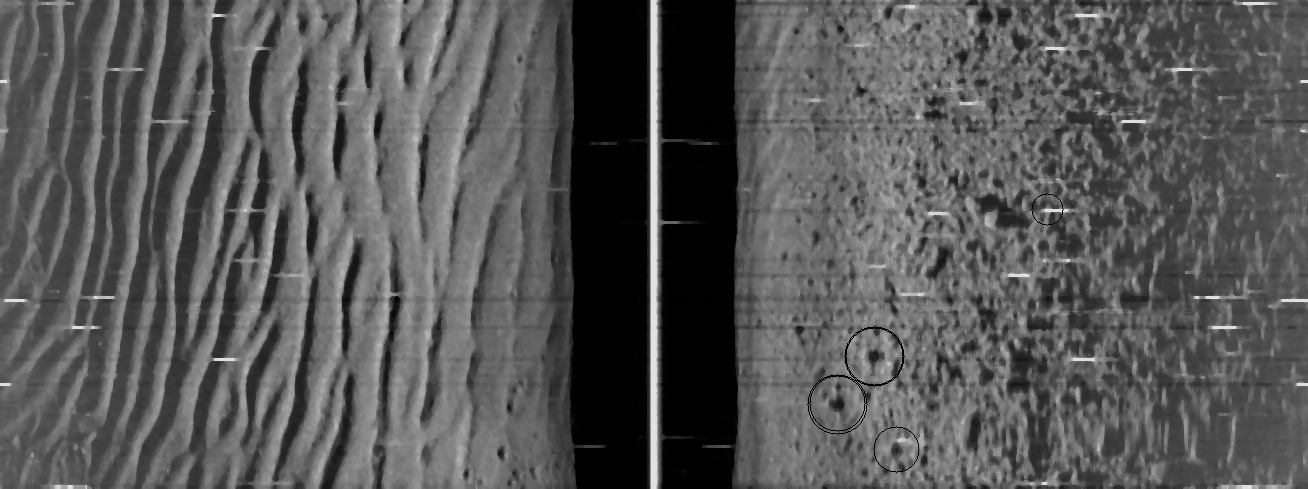
\includegraphics[width = 2.75 in]{/home/rohan/Documents/thesis/thesis_writeup/image_matched_sift.jpg}}\qquad
 \caption{\label{fig- matched images}Two consecutive side sonar images. The white circles represent the landmarks and the black circle in next image shows the matched keypoints.}
\end{figure}

The method to estimate motion is a very simple one with assumptions that AUV moves in a straight line at the same depth. To overcome the assumptions there needs to be work done on integrating side scan sonar pose in the algorithm. The method proposed in the section was to verify the dynamic landmark approach instead of proposing an algorithm for estimating motion. 

The performance of the algorithm is evaluated on real side sonar data. The results of the algorithm are compared to real motion information of the AUV and are discussed in the next chapter. 

\chapter{Results}
\label{ch-: results motion estimation}
\section{Motion estimation using side sonar images}
We validate our algorithm on datasets consisting of side sonar images
and the total distance the AUV moves.

{working on plotting the results}


\chapter{Conclusion}

Did it!

\bibliographystyle{plain}
\bibliography{mendeley.bib}

\end{document}
